\documentclass[11pt,english]{article}
\usepackage{NotesTeX}
\usepackage{mathpazo}

\usepackage{amsmath,amsthm,amssymb,bbm,mathtools,physics}
%\usepackage{braket}
\usepackage{graphicx}
\graphicspath{ {fig/} }
\usepackage[all]{xy}
\usepackage{tikz}
\usepackage{array}
\usepackage{dashrule}
\usepackage{changepage}
%\usepackage{floatrow}
\usepackage{epigraph} % inspirational quotes
\usepackage{cancel}
\usepackage{tcolorbox}
\usepackage{multirow}
\usepackage{empheq}
\usepackage{comment}
\usepackage{arydshln}

\usepackage{xcolor}
%\usepackage[breaklinks=true]{hyperref}
%\hypersetup{
	%  colorlinks   = true, %Colours links instead of ugly boxes
	%  urlcolor     = blue, %Colour for external hyperlinks
	%  linkcolor    = blue, %Colour of internal links
	%  citecolor   = magenta %Colour of citations
	%}
\definecolor{darkmagenta}{rgb}{0.55, 0.0, 0.55}
\definecolor{maincolor}{rgb}{0.8, 0.33, 0.0} % burnt orange แสด มน.
\definecolor{eqcolor}{rgb}{0.0, 0.447, 0.737} % french blue

\newcommand*{\eqbox}{%
	\tcboxmath[colback=eqcolor!10!white, colframe=eqcolor!95!black, size=fbox, arc=3pt, boxrule=0.8pt]%
}
%\definecolor{mycolor}{rgb}{0.0, 0.29, 0.29}
\newtcolorbox{mybox}[1][]{colback=eqcolor!10!white, colframe=eqcolor!95!black, title=#1}

\newcommand\tikzmark[1]{\tikz[remember picture,overlay]\coordinate (#1);}

	
\makeatletter

%\newcommand{\ketbra}[2]{\ket{#1}\bra{#2}}
\newcommand\dgg{^{\dagger}}
%\newcommand\Tr{\mathrm{Tr}}
\newcommand\id{\mathbbm{1}}
\newcommand\Id{\hat\mathbf{I}}
\newcommand\hilb{\mathcal{H}}
%\newcommand\abs[1]{\left|#1\right|}
\newcommand\av[1]{\left\langle #1 \right\rangle}
\newcommand\conj[1]{#1^*}
\newcommand{\R}{\mathbb R}
\newcommand{\C}{\mathbb C}
\newcommand{\Z}{\mathbb Z}
\newcommand{\E}{\mathbb E}

\renewcommand\op[1]{\widehat{#1}} % op in physics package is ketbra/dyad 
\newcommand\vecop[1]{\widehat{\boldsymbol{#1}}}
\newcommand\unc[1]{\hat #1_{\Delta}}
\newcommand\wunc[1]{\widehat #1_{\Delta}} 
% widehat for commonly used operators
\newcommand\bigzero{\makebox(0,0){\text{\huge0}}}
\renewcommand\H{\widehat H}
\newcommand\U{\widehat U}
\newcommand{\unit}[1]{\hat{\boldsymbol{#1}}}

\definecolor{strcyan}{RGB}{33,140,141}
\newcommand\todo[1]{{\color{strcyan} #1}}

%\@addtoreset{section}{part}
% equation numbering by chapters, not sections
%\numberwithin{equation}{part}
%\renewcommand{\theequation}{\arabic{part}.\arabic{equation}} 

%\newtheorem{theorem}{Theorem}[section]
\newtheorem{proposition}{Proposition}[section]
%\newtheorem{definition}{Definition}[section]
\theoremstyle{remark}
%\newtheorem{example}{Example}[section]% Example
\newcommand\mnf[1]{\marginnote{\footnotesize{#1}}}

\usepackage{pifont}
\newcommand{\xmark}{\text{\ding{55}}}
\newcommand\dashing{\noindent\vspace{-1ex}\makebox[\linewidth][r]{\hdashrule[1ex][x]{\textwidth}{0.4pt}{1pt 2pt}}}
%-----------------
\newcommand\red[1]{{\color{red} #1}}



%%%%%%%%%%%%%%%%%%%%%%%%%%%%%% Textclass specific LaTeX commands.
\newcommand{\lyxaddress}[1]{
	\par {\raggedright #1
		\vspace{1.4em}
		\noindent\par}
}


\makeatother

	\title{{Quantum Information}\\{\normalsize{\itshape }}}
	
	\author{Ninnat Dangniam}
	\affiliation{
		Institute for Fundamental Study (IF) \\
		Naresuan University,
		Phitsanulok, \\ Thailand 65000}
	\emailAdd{ninnatd@nu.ac.th}	
	
\begin{document}	
	
\maketitle

%===============================
%------------------------------
\section{Information and Bits}
%------------------------------
%===============================

%Information as defined by Claude Shannon is a statistical concept. Alternatives

%---------------------------------------------
\subsection{Probability}
%---------------------------------------------

We will set up and formalize notations to talk about randomness using the context of statistical experiments. These can be actual (``artificial") experiments in the lab, or natural processes, the outcomes of which are random.

Denote by $\Omega$ the set of all possible outcomes ({\bf events}) of a statistical experiment, usually called the {\bf sample space} or the ``universe".

%Let $\Omega$ be the set of all possible outcomes of a statistical experiment, also known as the {\bf sample space} or the ``universe".

\begin{example}[\bf Coin toss]\leavevmode
	The sample space consists of the outcome that the coin comes up head (H) or tail (T): $\Omega = \{H,T\}$.
\end{example} 
\begin{example}[\bf Die roll]\leavevmode
	The sample space is the number on the face of a die: $\Omega = \{1,2,3,4,5,6\}$.
\end{example}
\begin{margintable}
	\begin{tabular}{ |c|c|c| } 
		\hline
		& \multicolumn{1}{|p{1cm}|}{\centering \scriptsize{Logical} \\ \scriptsize{operation}} & \multicolumn{1}{|p{1cm}|}{\centering \scriptsize{Set} \\ \scriptsize{operation}}  \\
		\hline 
		NOT & $\neg A$ & $\overline{A}$ \\ 
		AND & $A \wedge B$ & $A \cap B$ \\
		OR & $A \vee B$ & $A \cup B$	\\
		\hline
	\end{tabular}
	\caption{Symbols for elementary logical operations and the corresponding set operations, which we use interchangeably.}
	\label{table:logical_operations}
\end{margintable}
Each outcome of a statistical experiment can be associated with a {\bf logical proposition} in the obvious way. For example, the result ``1" of a die roll is associated with the proposition ``the die is rolled and we obtained a 1". Every such proposition can be assigned a binary value TRUE or FALSE. 
These outcomes do not exhaust all possible events because we can combine events using logical (Boolean) operations such as AND or OR to create new logical propositions.


An {\bf empty event} (set) is denoted by $\emptyset$. Self-evidently,
\begin{align}
	A \wedge \overline{A} = \emptyset, && A \vee \overline{A} = \Omega.
\end{align}

Whenever $\Omega$ is a finite set, we can always find an elementary set of disjoint ({\bf mutually exclusive}) propositions called {\bf elementary events} or {\bf atomic events} $\{E_j\}_j$: %(These are nothing but the outcomes of our statistical experiment.) 
\begin{align}
	E_j \wedge E_k = \begin{cases}
		E_j, & j=k, \\
		\emptyset, & j\neq k.
	\end{cases}
\end{align}
The set of all possible events i.e. logical combinations of all atomic events, constitutes a \emph{Boolean algebra} $\{0,1\}^n$ whose size is $2^n$ if there are $n$ atomic events.
It is the set $\{0,1\}^n$ because an event is defined by whether each atomic event is absent or present in the Boolean formula $E_{j_1} \vee E_{j_2} \vee \cdots \vee E_{j_m}$, $m \le n$.
\begin{marginfigure}
	\centering
	\begin{tikzpicture}
		\node (max) at (0,4) {$\Omega$};
		\node (a) at (-2,2) {$B\vee C$};
		\node (b) at (0,2) {$A\vee C$};
		\node (c) at (2,2) {$A\vee B$};
		\node (d) at (-2,0) {$A$};
		\node (e) at (0,0) {$B$};
		\node (f) at (2,0) {$C$};
		\node (min) at (0,-2) {$\emptyset$};
		\draw (min) -- (d) -- (a) -- (max) -- (b) -- (f)
		(e) -- (min) -- (f) -- (c) -- (max)
		(d) -- (b);
		\draw[preaction={draw=white, -,line width=6pt}] (a) -- (e) -- (c);
	\end{tikzpicture}
	\label{}
	\caption{The Hesse diagram of a Boolean algebra with three atomic events $A, B$, and $C$. Going up in the diagram corresponds to the logical operation OR ($\vee$), while going down corresponds to AND ($\wedge$).}
\end{marginfigure}

\begin{mybox}
	 $\{0,1\}^n$ is also the \emph{power set} $\mathcal{P}(\Omega)$, the set of all subsets of $\Omega$.
	The power set $X^Y$ is the set of all functions from $Y$ to $X$. There are exactly $|X|^{|Y|}$ such functions, hence the notation. (Why? For each input in $Y$, one can choose an output from all possible choices of $x\in X$.)
\end{mybox}

So far we have not yet talked about assigning probabilities to events. There is a long-standing debate about what a probability actually means, but for us a probability is just a number between 0 (the event never occurs) and 1 (the event occurs with certainty).

\begin{definition}[\bf Probability axioms]\leavevmode
	
	\begin{enumerate}
		\item $\Pr(A) \ge 0$,
		\item $\Pr(A) =1 \iff A$ is certain,
		\item $\Pr(A\vee B) = \Pr(A)+\Pr(B)$ if $A\wedge B  =\emptyset$
	\end{enumerate}
\end{definition}
These axioms are sufficient to derive any other identities such as 
\begin{align}
	\Pr(\neg A) &= 1-\Pr(A), \\
	\Pr(A\vee B) &= \Pr(A) + \Pr(B) - \Pr(A\wedge B).
\end{align}

Let us formalize one more thing: a {\bf random variable} $X$ is a variable that takes a value $x\in \Omega$ with probability $\Pr(X=x)$. We usually write $X\sim f$ to mean that values of $X$ are distributed according to a probability distribution $f$.
\begin{align*}
	\boxed{\textrm{Random variable} \leftrightarrow \textrm{Statistical experiment}}
\end{align*}
We will use interchangeably the notations 
\begin{align}
	\Pr(X=x) \equiv p_X(x) \equiv p(x).
\end{align}
\begin{definition}[\bf $k$th moment]\leavevmode
	\begin{align}
		{\color{magenta}\underbracket{\color{black}\E[X^k]}_{\mathclap{\substack{\textrm{Mathema-} \\ \textrm{ticians'} \\ \textrm{notation}}}}} \equiv {\color{teal}\underbracket{\color{black}\av{X^k}}_{\mathclap{\substack{\textrm{Physicists'} \\ \textrm{notation}}}}}
		\equiv \av{x^k} = \sum_x x^k p(x)
	\end{align}
\end{definition}
\noindent The {\bf mean value}, also known as the average or the expectation value, is the first moment, whereas
the {\bf variance} is the part of the second moment that is independent of the first moment.\mn{The variance is the second \href{https://en.wikipedia.org/wiki/Cumulant}{cumulant}. The Gaussian distribution is the unique probability distribution whose cumulants all vanish except the first and the second.} 
\begin{align}
	\textrm{Var}(X) \equiv \sigma_x^2 = \av{(X-\av{X})}^2 = \av{X^2} - \av{X}^2
\end{align}

\begin{example}[\bf Bernoulli trials]\leavevmode
	
	Suppose that $X$ takes values $n$, the number of heads obtained in $N$ independent tosses of a coin with a bias $p$. (More about independence later.) The probability of such an event is given by the \emph{binomial distribution} $X\sim B(N,p)$. 
	
	\begin{align}
	\left(\parbox{8em}{\centering Probability of obtaining a particular sequence with exactly $n$ heads}\right) &= p^n(1-p)^{N-n} \\
	\Pr(X=n)  = \left(\parbox{8em}{\centering Probability of obtaining \emph{any} particular sequence with exactly $n$ heads}\right) &= {N \choose n}p^n(1-p)^{N-n}
	\end{align}

	The normalization can be verified directly. Let $q=1-p$.
	\begin{align}
		\sum_{n=0}^N \Pr(X=n) = \sum_{n=0}^N{N \choose n}p^n q^{N-n} 
		= (p+q)^N = 1,
	\end{align}
	where we have used the binomial theorem in the second-to-last equality.
	\begin{align}
		\av{n} &= \sum_{n=0}^N np(n) = \sum_{n=0}^N n{N \choose n}p^n q^{N-n} \\
		&= p \pdv{p}\sum_{n=0}^N {N \choose n}p^n q^{N-n}
		= p \pdv{p}(p+q)^N \\
		&= Np \cancelto{1}{(p+q)^{N-1}} = Np
	\end{align}
	The same trick can be used to calculate the variance  $\sigma^2 = Np(1-p)$.
\end{example}


%---------------------------------------------
%\subsection{Correlation}
%---------------------------------------------

Things become interesting when there are two or more random variables.
\begin{definition}[\bf Joint probability]\leavevmode
	\begin{align}
		\Pr(X=x,Y=y) \equiv p_{XY}(x,y) \equiv p(x,y)
	\end{align} 
	is the probability that both the outcomes $x$ and $y$ happen.
\end{definition}

\begin{definition}[\bf Marginal probability]\leavevmode
	\mnf{\begin{align}
			p(x) = {\color{maincolor}\underbracket{\color{black}p(x,y)}_{\mathclap{\substack{ \textrm{Probability} \\ \textrm{that both $x$} \\ \textrm{and $y$ occur} }}} } 
			\; + \; {\color{eqcolor}\underbracket{\color{black}p(x,\neg y)}_{\mathclap{\substack{\textrm{Probability} \\ \textrm{that $x$ occurs} \\ \textrm{but $y$ doesn't} }}} }
	\end{align}} 
	\begin{align}
		p(x) = \sum_y p(x,y), && p(y) = \sum_x p(x,y),
	\end{align}
\end{definition}
\noindent A marginal probability is the probability that an outcome described by one of the random variables may occur without looking at the outcome of the other random variable.

\begin{definition}[\bf Conditional probability]\leavevmode
		
	For $\Pr(Y=y) \neq 0$,
	\begin{align}
		\Pr(\smash{X=x|\underbracket{Y=y}_{\textrm{Condition}}}) \equiv p(x|y) = \frac{p(x,y)}{p(y)}
	\end{align}
	is the probability that the event $x$ occurs \emph{if} the event $y$ also occurs.
\end{definition}
\noindent A conditional probability distribution for a fixed value of $Y$ must normalize to 1.
\begin{align}
	\sum_x p(x|y) = \frac{1}{p(y)} \sum_x p(x,y) = \frac{\cancel{p(y)}}{\cancel{p(y)}} = 1
\end{align}
Other useful equalities are obtained from these basic definitions.
\begin{lemma}[\bf Law of total probability]\leavevmode
	\begin{align}
		p(x) = \sum_y p(x|y)p(y)
	\end{align}
\end{lemma}

\begin{lemma}[\bf Bayes' theorem]\leavevmode
	\begin{align}
		p(x|y) = \frac{p(y|x)p(x)}{p(y)}.
	\end{align}
\end{lemma}
\noindent Bayes' theorem emphasizes that $p(x|y)$ and $p(y|x)$ are not equal in general. As an example, the probability of having Covid given a positive test result is not equivalent to the probability of testing positive when actually having Covid.
Usually when computing $p(x|y)$ via Bayes' theorem, one computes the denominator $p(y)$ using the law of total probability.

\begin{definition}
	Events $x$ and $y$ are {\bf independent} if 
	\begin{align}
		p(x,y) = p(x)p(y).
	\end{align}
	Otherwise, they are {\bf correlated}. We also say that two random variables $X$ and $Y$ are correlated if $p(x,y) \neq p(x)p(y)$ for some $x$ and $y$.
\end{definition}
\noindent In words, events $x$ and $y$ are independent if looking at the outcome of one of them does not give you any information about the other event i.e. does not make the other event more or less likely to occur.
\begin{align}
	p(x|y) = \frac{p(x,y)}{p(y)} = \frac{p(x)\cancel{p(y)}}{\cancel{p(y)}} = p(x).
\end{align}

\begin{mybox}
Mutually exclusive events cannot be independent. If I flip a coin and it comes up head, it could not have come up tail. Mathematically, this is because, if $x\wedge y =\emptyset$, then $p(x,y)=0$ but $p(x)p(y)$ cannot be zero if both $p(x)$ and $p(y)$ are nonzero.
\end{mybox}

%---------------------------------------------
\subsection{Information entropy}
%---------------------------------------------

The number of bits required to describe a random variable is quantified by the Shannon entropy.
\begin{definition}[\bf Shannon entropy]\leavevmode
	\begin{align}
		H(X) \equiv -\sum_x p(x) \log p(x)
	\end{align} 
\end{definition}
\noindent When the logarithm is base 2, the entropy is measured in terms of \emph{bits}. The special case when all $n$ outcomes are equally likely reduces $H(X)$ to the Hartley entropy $\log n$. In physics, sometimes the natural log is used\mn{It is still common, however, to use logarithm base 2 in quantum information science.} and the Shannon entropy is proportional to the Gibbs entropy, which reduces to the Boltzmann entropy in the case of the uniform distribution.

Think of the Shannon entropy as the average \emph{surprisal}, $-\log p(x)$, upon learning an outcome $x$. The rarer the outcome $x$ is, the more information you gain by observing $x$ occurring.\mn{You may be worried that $-\log 0=\infty$, but one can show that $\lim_{x\to 0^+} 0 \log 0=0$ by L'hospital's rule.} Also worth noting is that $\log 1 = 0$ agrees with our intuition that an observation can only convey new information when there are alternatives to the outcome that we have observed.


\begin{example}[\bf Horse race]\leavevmode
	
An example that illustrates how the Shannon entropy determines the amount of information in a random source is the following.
\vspace{0.5em}

Consider a scenario where you agree to watch a horse race and send a telegram to your friend, indicating the winning horse while minimizing the number of letters used in the message. 
Suppose that there are four horses in the race, and you and your friend believe that the chance of horse \#1 winning is 1/2, horse \#2 winning is 1/4, and horses \#3 and \#4 winning are equally likely at 1/8 each.
\vspace{0.5em}

A naive encoding protocol would be to assign two bits to represent each horses: 00 for horse \#1, 01 for horse \#2, 10 for horse \#3, and 11 for horse \#4. However, there is a more efficient way to achieve a better average message length by utilizing a \emph{variable-length} code. To ensure unique decodability, you may want to use, say, a prefix-free code where no codeword is a prefix of another. In this case, you can encode the horses as follows: 0 for horse \#1, 10 for horse \#2, 110 for horse \#3, and 111 for horse \#4. The average length of this encoding is
\begin{align}
	1\cdot \frac{1}{2} + 2\cdot \frac{1}{4} + 2\cdot 3\cdot \frac{1}{8} = 1.75 <2. 
\end{align}
Notice that the computation of the average message length is precisely the computation of the Shannon entropy. In fact, by an application of \href{https://en.wikipedia.org/wiki/Kraft%E2%80%93McMillan_inequality}{Kraft inequality}, one can show that the Shannon entropy upper bounds the expected length of any prefix-free code. Also, by thinking about   \href{https://en.wikipedia.org/wiki/Huffman_coding}{Huffman coding} which achieves the optimal expected message length, one can also see that the Shannon entropy gives the expected number of binary questions one needs to ask to completely remove the uncertainty from a random variable.
\end{example}

\begin{example}[\bf Typical sequences]\leavevmode
	
	Consider a multinomial distribution which generalizes the binomial distribution to $d$ outcomes.
	\begin{align}
		p(n_1,n_2,\dots,n_d) = \frac{N!}{n_1!\cdots n_d!} p_1^{n_1} \cdots p_d^{n_d}.	
	\end{align}
	In the limit of a long-running experiment $N\to\infty$, the number of $x_j$ that appears in a sequence is $\av{n_j} = Np_j$. A sequence in which $x_j$ appears exactly $\av{n_j}$ times is said to be a \emph{typical sequence}.
	\begin{align}
		\left(\parbox{8em}{\centering Probability of obtaining a particular typical sequence}\right) &= p_1^{n_1} \cdots p_d^{n_d} 
		= p_1^{Np_1} \cdots p_d^{Np_d} \\
		&= \exp(Np_1\log p_1) \cdots \exp(Np_d\log p_d) \\
		&= \exp[N(p_1 \log p_1 + \cdots + p_d \log p_d)] \\
		&= e^{-NH(X)}
	\end{align}
	If we count the number of such a typical sequence, we will find that
	\begin{align}
		\ln\left(\frac{N!}{n_1!\cdots n_d!}\right)
		&= \ln (N!) - \sum_j \ln (n_j!) \\
		&= N\ln N - \cancel{N} - \sum_j (n_j \ln n_j - \cancel{n_j}) \mnf{Stirling's formula} \\
		&= N\ln N - \sum_j Np_j \ln (Np_j) \\
		&= \cancel{N\ln N} - \cancel{N\ln N} - N\sum_j p_j \log p_j \\
		&= NH(X).
	\end{align}
	Remarkably, each typical sequence appears with probability $e^{-NH(X)}$ and there are $e^{NH(X)}$ of them, so they monopolize all the probabilities. This \emph{asymptotic equipartition property} lies at the heart of Shannon's information theory.
\end{example}

\begin{definition}[\bf Joint entropy]\leavevmode
	\begin{align}
		H(X,Y) = -\sum_{xy} p(x,y) \log p(x,y)
	\end{align}
\end{definition}

\begin{definition}[\bf Conditional entropy]\leavevmode
	Since $p(x|y)$ defines a probability distribution for a fixed $y$. Let
	\begin{align}
		H(X|Y=y) \equiv -\sum_x p(x|y)\log p(x|y).
	\end{align}
	Then the conditional entropy is the average
	\begin{align}
		H(X|Y) = \sum_y p(y)H(X|Y=y).
	\end{align}
\end{definition}

\begin{lemma}\label{}
	\begin{align}
		H(X|Y) = H(X,Y) - H(Y)
	\end{align}
	In words, the conditional entropy is the uncertainty left in $X$ after observing the value of $Y$.
\end{lemma}
	
\begin{align}
	H(X|Y) &= \sum_y p(y)H(X|Y=y) 
		= \sum_y p(y) \sum_x p(x|y) \log p(x|y) \\
		&= -\sum_{xy} p(x,y) [\log p(x,y)-\log p(y)] \\
		&= H(X,Y) + \sum_y \underbrace{\sum_x p(x,y)}_{p(y)} \log p(y) 
		= \boxed{H(X,Y) - H(Y)}
\end{align}

\begin{definition}[\bf Mutual information]\leavevmode
	The common information shared between $X$ and $Y$ is
	\begin{align}
		H(X:Y) &= \sum_{x,y}p(x,y)\log\left(\frac{p(x,y)}{p(x)p(y)}\right) \\
			&= H(X) + H(Y) - H(X,Y)
	\end{align}
\end{definition}

\begin{figure}[h]
	\centering
	\label{}
	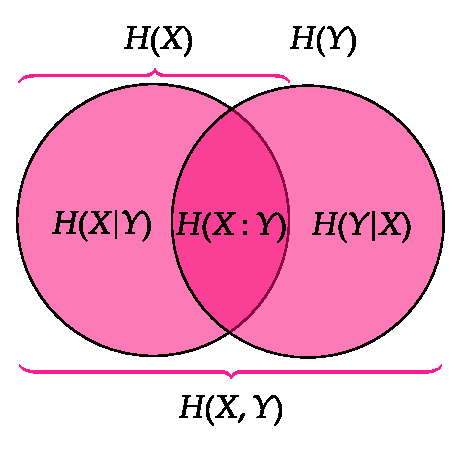
\includegraphics[scale=0.8]{fig/venn-entropy.pdf}
	\caption{Venn diagram showing the relationships between various entropic quantities associated with two random variables.}
\end{figure}

\newpage

%===============================
%------------------------------
\section{Mathematical Prerequisite}
%------------------------------
%===============================


%---------------------------------------------
\subsection{Transition from wave mechanics}
%---------------------------------------------



The stationary states from a complete, orthonormal set
\begin{empheq}[box=\fbox]{align}
	\int dx\, \varphi_n^* (x) \varphi_m(x) &= \delta_{nm}
	\mnf{Orthonormality} \label{eq:orthogonality-function-space}  \\
\sum_{n} \varphi_n^*(x) \varphi_n(x') &= \delta(x-x')
\mnf{Completeness \mbox{(Closure relation)}} \label{eq:completeness-function-space}
\end{empheq}
The Dirac delta ``function" is a generalized function, also known as a distribution, and only has meaning inside an integral.
\begin{align}
	\int dx'\, f(x') \delta(x-x') = f(x)
\end{align}
Think of the delta function as a linear map from $\hilb$ to $\C$.

Given a function $\psi(x)$. Suppose that we can write
\begin{align}\label{eq:expansion-function-space}
	\psi(x) &= \sum_n c_n \varphi_n(x).
\end{align}
Orthogonality implies that
\begin{align}
	\int dx\, \varphi_n^*(x)\psi(x) 
	&= \sum_m c_m \int dx\, \varphi^*_n(x)\varphi_m(x)  \\
	&= \sum_m c_m \delta_{nm} = c_n.
\end{align}
In other words, we have an identity
\begin{align}
	\boxed{c_n = \int dx\, \varphi_n^*(x)\psi(x) }\,.
\end{align}
Equipped with the orthonormality relation, we can show that the closure relation is equivalent to the spanning property.\mn{Of course, a set that is not orthonormal (nor orthogonal) can also span the space, in which case the closure relation is generalized to the \href{https://en.wikipedia.org/wiki/Frame_(linear_algebra)}{\emph{frame condition}}.}
\begin{lemma}\label{}
	An orthonormal set $\{\varphi_n(x)\}_n$ spans the space of function if and only if it satisfies the closure relation \eqref{eq:completeness-function-space}.
\end{lemma}
\begin{proof}
	``$\impliedby$" direction
	
	Suppose that the closure relation is true. For an arbitrary $\psi(x)$, compute $\psi(x) = \sum_n c_n \varphi_n(x)$. We want to show that $\sum_nc_n\varphi_n(x)$ is nothing but $\psi(x)$.
	\begin{align}
		\sum_nc_n\varphi_n(x) &= \int dx'\, \psi(x') \sum_n \varphi_n^*(x') \varphi_n(x) \\
		&= \int dx'\, \psi(x')\delta(x-x') = \psi(x)
	\end{align}
	as desired.
	
	``$\implies$" direction
	
	Suppose that the expansion \eqref{eq:expansion-function-space} is valid for an arbitrary function,
	\begin{align}
		\psi(x) &=  \int dx'\, \psi(x') \sum_n \varphi_n^*(x') \varphi_n(x),  
	\end{align}
	then it must be that the sum acts like a Dirac delta function, which completes the proof.
\end{proof}

In quantum theory, $\abs{c_n}^2$ has the meaning of the probability to find the system in the state $\varphi_n(x)$. It is straightforward to verify that
\begin{align}
	\sum_n \abs{c_n}^2 = \int dx\, \abs{\psi(x)}^2.
\end{align}
More generally, if $\psi(x) = \sum_n c_n \varphi_n(x)$ and $\phi(x) = \sum_n d_n \varphi_n(x)$. Then the inner product in the function space is the same as the inner product between infinitely long vectors of sequences $\{c_n\}_n$ and $\{d_n\}_n$:
\begin{align}
	\int dx\, \phi^*(x)\psi(x) &= \sum_{nm} d_n^* c_m \int dx\, \varphi_n^*(x) \varphi_m(x) \\
	&= \sum_{nm} d_n^* c_m \delta_{nm} = \sum_n d_n^* c_n \\
	&= \mqty(d_1^*&d_2^*&\dots)\mqty(c_1\\c_2\\ \vdots)
\end{align}
Technically, these two kinds of inner product define different Hilbert spaces. One is the space $l^2$ of \emph{square-summable} sequences, 
\begin{align}
	\sum_n \abs{c_n}^2 < \infty.
\end{align}
The other is the space $L^2$ of \emph{square-integrable} functions, 
\begin{align}
	\int dx\, \abs{\psi(x)}^2 < \infty.
\end{align}

In Heisenberg's original conception of quantum theory, he rejected ascribing (continuous-valued) dynamical variables such as position and momentum to atomic orbitals on the basis that they are unobservable and that a theory that included them so far had failed to make the correct prediction \cite{jammer}. 
Heisenberg focused instead on discrete quantities $n=1,2,\dots$ that label the atomic orbitals.
In this approach, known as \emph{matrix mechanics}, there are only observables and ``quantum jumps" between different values of an observable. 
Notably, there is no notion of a quantum state\mn{So one is spared from having to physically interpret a superposition of quantum states.}, but one can think of the coefficients $\{c_n\}_n$ as a ``state". Thus, one is working in the Hilbert space $l^2$ of square-summable sequences.

Schr\"odinger came from a different vantage point entirely. He took seriously de Broglie's idea that associated to every quantum particle is a wave and asked what the wave equation for de Broglie's waves are. This led to the Schr\"odinger equation and the approach known as \emph{wave mechanics}. 
In this approach, there are only states, but no probability, at least at first.\mn{Schr\"odinger hihmself even mistakenly believed that the wave function describes a charge density of some sort.} 
It was Max Born that supplemented the probabilistic interpretation in this approach. As a result, one is working in the Hilbert space $L^2$ of square-integrable functions.

However, the two approaches were the same all along as the two Hilbert spaces are equivalent (Riesz-Fischer theorem).
From this line of thinking, John von Neumann developed a unified formulation of quantum mechanics as we know today \cite{landsman,jammer}. For us, the whole point is that $\{c_n\}_n$ and $\psi(x)$ are simply two representations of the same element  $\ket{\psi}$ of an abstract Hilbert space $\hilb$.

\begin{example}[Particle in a box]\leavevmode
	\begin{align}
		\ket{\varphi_n} \longleftrightarrow \varphi_n(x) = \sqrt{\frac{2}{L}} \cdot
		\begin{cases}
			 \sin(k_n x), & \textrm{even}\, n, \\
			 \cos(k_n x), & \textrm{odd}\, n,
		\end{cases}
	\end{align}
	where $k_n = n\pi/L$.
Note the important fact that the ket $\ket{\varphi_n}$ has no $x$-dependence.
\end{example}

\begin{example}[Spin-1/2]\leavevmode
	\begin{align}
		\ket{\psi} = \alpha\ket{\uparrow} + \beta\ket{\downarrow}
	\end{align}
\end{example}



%---------------------------------------------
\subsection{Inner product spaces}
%---------------------------------------------

The prerequisites of this section are definitions and basic properties related to vector spaces and linear operators, which can be found in Appendix \ref{sec:A01}.

%From a logical standpoint, finite and infinite-dimensional Hilbert spaces are the same. A finite-dimensional Hilbert space is a vector space equipped with an inner product.
\begin{definition}
A pairing
	\begin{align}
		V\times V &\to\C, \\
		\phi,\psi &\mapsto (\varphi,\psi)
	\end{align}
is said to be an {\bf inner product} if the following properties are satisfied.
	\begin{itemize}
		\item \emph{Linearity in the second argument}: 
		\begin{align}
			(\phi, a\psi_1 + b\psi_2) = a(\phi,\psi_1) + b(\phi,\psi_2) 
			\label{eq:inner-product-linearity}
		\end{align}
		\item \emph{Conjugate symmetry:}
		\begin{align}
			(\psi,\phi) = (\phi,\psi)^*
			\label{eq:inner-product-conjugate-symmetry} 
		\end{align}
		\item \emph{Positive-definiteness:} 
		\begin{align}
			(\psi,\psi) \ge 0 \;\textrm{with equality iff} \ket{\psi} = 0 
			\label{eq:inner-product-+ve-definite}
		\end{align}
	\end{itemize}
\end{definition}



Inner products in real vector spaces are bilinear, but inner products in complex vector spaces are  \emph{sesquilinear} they are , i.e., they are conjugate linear in the first argument. Sesquilinearity follows from \eqref{eq:inner-product-linearity} and \eqref{eq:inner-product-conjugate-symmetry}
\begin{align}
	(a\phi_1 + b\phi_2,\psi) &= (\psi,a\phi_1 + b\phi_2)^* \\
		&= a^*(\psi,\phi_1)^* + b^*(\psi,\phi_2)^* \\
		&= a^* (\phi_1,\psi) + b^*(\phi_2,\psi) 
\end{align}
Sesquilinearity is required to make $(\psi,\psi)$ non-negative. %We will see that sesquilinearity has consequence to how we define the adjoint of a linear operator, from which the whole business about the spectral theorem slides down.

\begin{example}[Weird inner product]\leavevmode
	
	The following formula defines an inner product in $\R^2$.
	\begin{align}
		(x,y) = 5x_1y_1 + x_1y_2 + x_2y_1 + 3x_2y_2.
	\end{align}
	The positive definiteness can be shown by noting that
	\begin{align}
		(x,x) = 5x_1^2 + 2x_1x_2 + 3x_2^2 = (x_1+x_2)^2 + 4x_1^2 + 2x_2^2 \ge 0,
	\end{align}
	with equality iff every term is zero.
\end{example}

%Obviously the dot product is an inner product. But is there anything else? An inner product can be equivalently given by a bilinear form (or sesquilinear in complex vector spaces).

An inner product with a fixed vector $\phi$ always can be thought as a mapping
\begin{align}
	(\phi, \_ \,): V &\to \C, \\
	\psi &\mapsto (\phi,\psi)
\end{align}
This is an example of a \emph{linear functional}, a linear map from $V$ to $\C$.
%This is a linear map from a vector space $\hilb$ to the one-dimensional vector space $\C$. Thus, it can be represented by  a 1-by-d matrix.

\begin{definition}
	The {\bf dual space} $V^*$ of $V$ is defined as the vector space of linear functionals with addition defined as\mn{Scalar multiplication in $V^*$ follows directly from the the linearity of linear functionals: $f(a\psi)=af(\psi)$.}
	\begin{align}
		(f+g)(\psi) = f(\psi) + g(\psi).
	\end{align} 
	%Furthermore, we write the action of any linear functional $f\in V^*$ on $\ket{\psi} \in V$ as
	%\begin{align}
	%	\av{f|\psi} \equiv f(\psi).
	%\end{align}
	%$\bra{f}$ is called a {\bf bra}.
	 %represented by bras $\bra{\phi}$. 
\end{definition}

\begin{lemma}
	$\dim V^* = \dim V$.
\end{lemma}
%\noindent A formal proof can be given as follows.
\begin{proof}	
	For any given basis $\{e_j\}_j$ for $V$, we can define a basis $\{f_k\}_k$ for $V^*$ by the relation $f_k(e_j) = \delta_{jk}$. If there is an element $g$ of $V^*$ that cannot be represented as a linear combination of $\{f_k\}_k$, then $g(e_j) = 0$ for every $j$, which implies that $g$ is the zero map. Therefore, $\{f_k\}_k$ spans $V^*$ and there are $\dim V$ of them.
\end{proof}
For finite dimensional vector spaces, the characterization of linear functionals are obvious in matrix form. By definition, any linear map from an $n$-dimensional vector space to $\C$ can be represented by a 1-by-$n$ matrix, 
\begin{align}
	f\left[\mqty(c_1\\c_2\\ \vdots \\ c_n)\right] = \mqty(* & * &\dots & *) \mqty(c_1\\c_2\\ \vdots \\ c_n),
\end{align}
which suggests that all linear functionals can be realized as an inner product.\mn{But note that the notion of linear functionals of the dual space does not require the notion of an inner product.} 
This is indeed true (Riez representation theorem). An inner product induces an antilinear map $\dgg$ that identifies $V$ and $V^*$,
\begin{align}
	\ket{\psi} \overset{\dagger}{\longleftrightarrow} \bra{\psi}, 
\end{align}
but the specification of the map itself will depend on the choice of the inner product. If we choose an orthonormal basis $\{\ket{e_j}\}_{j=1}^n$,
\begin{align}
	(e_j,e_k) = \delta_{jk},
\end{align} 
this map is
\begin{align}
	c_1 \ket{e_1} + \dots + c_n\ket{e_n} \overset{\dagger}{\longleftrightarrow} 
		c_1^* \bra{e_1} + \dots + c_n^*\bra{e_n}.
\end{align}
In other words, $f \in V^*$ is identified with the vector $\phi_f = \sum_j[f(e_j)]^* e_j \in V$, for suppose that $\psi = \sum_j c_j e_j$, then
\begin{align}
	(\phi_f,\psi) &= \sum_j c_j (v_f,e_j) \mnf{Linearity in the second argument} \\
	&= \sum_{jk} c_j  \{[f(e_k)]^*\}^* (e_k,e_j) = \sum_{jk} c_j  [f(e_k)] \delta_{jk} \mnf{Conjugate linearity in the first argument} \\
	&= \sum_j c_j f(e_j) = f\left[\sum_j c_j e_j\right] = f(\psi),
\end{align}
as it should be.



\begin{theorem}[\bf Cauchy-Schwarz]\leavevmode\label{thm:CS-ineq}

$$\abs{\braket{\phi}{\psi}}^2 \le \braket{\phi} \braket{\psi}$$
\end{theorem}

\begin{marginfigure}
	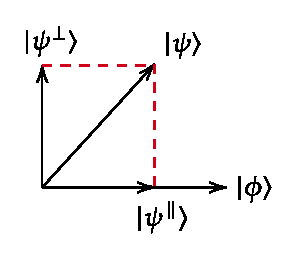
\includegraphics[scale=1]{fig/pythagorean.pdf}
	\caption{}
	\label{fig:pythagorean}
\end{marginfigure}
\begin{proof}
	Given a pair of vectors $\ket{\phi}$ and $\ket{\psi}$, one can consider the triangle formed by $\ket{\psi^{\parallel}}$, the component of $\ket{\psi}$ parallel to $\ket{\phi}$:
	\begin{align}
		\ket*{\psi^{\parallel}} = 
		\frac{\av{\phi|\psi}}{\av{\phi|\phi}}\ket{\phi}, 
	\end{align}
	and the perpendicular component $\ket{\psi^{\perp}} = \ket{\psi} - \ket*{\psi^{\parallel}}$, see Fig \ref{fig:pythagorean}.
	
	
	The Pythagorean theorem tells us that
	\begin{align}
		\braket{\psi}  &= \braket*{\psi^{\perp}} + \braket*{\psi^{\parallel}} \\
		\braket{\psi} - \frac{\abs{\braket{\phi}{\psi}}^2}{\braket{\phi}} &= \braket*{\psi^{\perp}} \ge 0
		\label{eq:pythagorean}.
	\end{align}
	from which the Cauchy-Schwarz inequality
	\begin{align}
		\abs{\av{\phi|\psi}}^2 &\le \av{\phi|\phi}\av{\psi|\psi}
	\end{align}
emerges.
	Additionally, we see from \eqref{eq:pythagorean} that the inequality is tight iff $\ket{\phi}$ and $\ket{\psi}$ are scalar multiple of each other.
\end{proof}

\begin{definition}
	The norm of $\ket{\psi}$ is $\norm{\ket{\psi}} \equiv \norm{\psi} \coloneqq \sqrt{\braket{\psi}}$.
\end{definition}
\noindent Since an inner product defines a norm, a Hilbert space is also a normed vector space.\mn{The converse is not true. Even though an inner product can be constructed from the 2-norm via the \href{https://en.wikipedia.org/wiki/Polarization_identity}{polarization identity}, (the $p$-norm is defined as $\norm{\psi}_p = \sqrt[p]{\sum \abs{c_j}^p}$), a normed space is not always an inner product space.  Take the max norm, $\norm{\psi}_{\infty} = \max_j \abs{c_j}$, for example.} By definition, a norm needs to satisfy the triangle inequality
\begin{align}
	\norm{\ket{\psi}+\ket{\phi}} \le \norm{\psi} + \norm{\phi}.
\end{align}
But for a norm induced from an inner product, the triangle inequality can be proved using the Cauchy-Schwarz inequality. Since the latter holds for any inner product, the former holds irrespective of the choice of inner product used to define the norm.
\begin{proof}
	\begin{align}
		\norm{\ket{\psi}+\ket{\phi}}^2 
		&= \norm{\psi}^2 + \norm{\phi}^2 + 2\mathrm{Re}\braket{\psi}{\phi} \\
		&\le \norm{\psi}^2 + \norm{\phi}^2 + 2\abs{\braket{\psi}{\phi}} \\
		&\le \norm{\psi}^2 + \norm{\phi}^2 + 2\norm{\psi}\cdot \norm{\phi}\mnf{Cauchy-Schwarz inequality} \\
		&= (\norm{\psi} + \norm{\phi})^2
	\end{align}
\end{proof}


The vector space in quantum theory is a \emph{separable Hilbert space}. A {\bf Hilbert space}, denoted by $\hilb$, is a vector space equipped with an inner product and some convergence properties. Separability means that there exists a countable basis for the space.\mn{Stationary states $\ket{\varphi}_n$ form a countable basis, but continuous eigenvectors such as $\ket{x}$ do not.} Additionally, since the norm of a vector has the meaning of a probability, we demand that the norm of every vector is finite. (As a consequence of the Cauchy-Schwarz inequality, this also means that every inner product is finite.) For a finite-dimensional vector space, all these issues about separability and finiteness of the norm never arises; in this case, a Hilbert space \emph{is simply an inner product space}.


\begin{mybox}
	Given the correspondence between linear functionals and the inner product, the \emph{bra-ket} $\av{v|u}$
	is often regarded as merely another notation for the inner product between two vectors in the Hilbert space.
	This interpretation is always valid in finite dimensions, but in an infinite-dimensional Hilbert space, there are linear functionals that have no corresponding vector. Take the bra $\bra{x}$, for example. Its squared norm is 
	\begin{align}
		\braket{x} = \int dx' \braket{x}{x'}\braket{x'}{x} = \int dx' \delta^2(x-x') = \delta(0) = \infty.
	\end{align}
\end{mybox}


Now we are ready to write down properties of an {\bf orthonormal basis (ONB)} in the Dirac notation. 
\begin{empheq}[box=\fbox]{align}
	\av{e_j|e_k} &= \delta_{jk}\label{eq:orthonormality} \mnf{Orthonormality} \\
\sum_j \dyad{e_j} &= \op \id \label{eq:completeness} \mnf{Completeness}
\end{empheq}
The equivalence of the spanning property and \eqref{eq:completeness} can be shown similar to the continuous case.
Suppose
\begin{align}
	\ket{\psi} = \sum_j c_j \ket{e_j}.
\end{align}
Then
\begin{align}
	\av{e_j|\psi} &= \sum_k c_k \av{e_j|e_k} \\
		&= \sum_k c_k \delta_{jk} = c_j.
\end{align}
That is, we have that
\begin{align}
	\boxed{c_j = \av{e_j|\psi}}\, .
\end{align}
Then suppose that an arbitrary vector can be expanded in such a way,
\begin{align}
	\ket{\psi} &= \sum_j c_j \ket{e_j} = \sum_j \ket{e_j}\av{e_j|\psi}. 
\end{align}
Then it must be the case that $\sum_j \dyad{e_j} = \hat \id$.




%---------------------------------------------
\subsection{Linear operators}
%---------------------------------------------

Any linear operator takes as an input a vector and outputs another vector. From this we observe that a ket-bra like $\dyad{\psi}{\phi}$ is a linear operator since
\begin{align}
	\ket{\psi}\av{\phi|\zeta} = \av{\phi|\zeta}\ket{\psi}, 
\end{align}
which is again a vector.\mn{In particular, the vector space of linear operators on $\hilb$ is $\hilb^* \otimes \hilb$.} This is the magic of the bra-ket notation. 


If an orthonormal set $\{\ket{\varphi_j}\}_j$ spans a subspace $S \subset V$, then 
\begin{align}
	\op P_S = \sum_j \dyad{e_j} 
\end{align}
is a projection operator onto the subspace $S$ and
$\op \id - \op P_S$
is the projection operator onto the orthogonal complement $S^{\perp}$. That is, the total space is the direct sum
$V = S \oplus S^{\perp}$,
and for $\ket v = \ket s + \ket p\in V$, where $s\in S$ and $p\in S^{\perp}$, we have that $\op P_S\ket v = \ket s$ and $(\op\id - \op P_S)\ket v = \ket p$.

\vspace{0.5em}
\noindent {\bf Matrix elements.}
\begin{align}
	\op T &= \hat\id \op T \hat\id = \sum_{jk} \ket{e_j} {\color{maincolor}\overbrace{\bra{e_j}\op T \ket{e_k}}^{T_{nm}}} \bra{e_k} 
\end{align}
\begin{align}
	\op T\ket{\psi} &= \sum_{jk} T_{jk} {\color{eqcolor}\overbrace{\av{e_k|\psi}}^{c_k}} = \sum_j {\color{darkmagenta}\overbrace{\left(\sum_k T_{jk}c_k \right)}^{d_j}} \ket{e_j} \\
	&\leftrightarrow \mqty(d_1 \\ d_2 \\  \vdots \\ d_n) = \mqty(T_{11}&T_{12}& \dots & & T_{1n} \\ T_{21}& T_{22} & & & \vdots \\ \vdots & & \ddots & & \\ T_{n1} & \dots & & & T_{nn})  \mqty(c_1 \\ c_2 \\ \vdots \\ c_n)
\end{align}
We see that the components transform as
\begin{align}\label{eq:transform-component}
	\boxed{d_j = \sum_k T_{jk} c_k}\,.
\end{align}
The transformation of basis vectors is in a sense ``opposite":
\begin{align}\label{eq:transform-basis}
	\boxed{\op T \ket{e_j} = \sum_k T_{kj}\ket{e_k}}.
\end{align}
The merit of the Dirac notation is that it streamlines matrix multiplications.
\begin{align}
	\op T \op S &= \sum_{jklm} T_{jl}S_{mk} \ket{e_j}\av{e_l|e_m}\bra{e_k}	
	= \sum_{jk} {\color{teal}\underbrace{\left(\sum_l T_{jl}S_{lk}\right)}_{(\op T \op S)_{nm}}}  \dyad{e_j}{e_k} 
\end{align}
For example, \eqref{eq:transform-basis} can be derived without breaking a sweat.
\begin{align}
	\op T\ket{e_j} &= \sum_{kl} T_{kl} \ket{e_k}\av{e_l|e_j} = \sum_{jk} T_{kj} \ket{e_k}
\end{align}
The same is true for \eqref{eq:transform-component}.
\begin{align}
	d_j &= \mel{e_j}{\op T}{\psi} = \sum_{klm} T_{kl} c_m \av{e_j|e_k} \av{e_l|e_m} 
		= \sum_l T_{jm} c_m 
\end{align}

\begin{comment}
	\vspace{0.5em}
	\noindent {\bf Commutator.}
	
	The commutator is 
	\begin{align}
		[\op A, \op B] = \op A \op B - \op B \op A.
	\end{align}
\end{comment}


\vspace{0.5em}
\noindent {\bf Trace.}
The manifestly basis-independent definition of the trace is 
\begin{align}
	\tr(\dyad{\psi}{\phi}) = \av{\phi|\psi},
\end{align}
which, in an ONB, equivalent to
\begin{align}
	\tr \op T &= \sum_{jk} T_{jk} \tr(\dyad{e_j}{e_k}) \mnf{Linearity of the trace} \\
	&= \sum_{jk}T_{jk} \av{e_k|e_j} = \sum_j T_{jj} = \sum_j \expval{\op T}{e_j}.
\end{align}
The trace has the cyclic property
\begin{align}
	\tr(\hat A \op B) = \tr(\op B \hat A).
\end{align}
Beware that for three or more matrices in the product, the cyclic property means that
\begin{align}
	\tr(\hat A \op B \op C) = \tr(\op B \op C \hat A),
\end{align}
whereas
\begin{align}
	\tr(\hat A \op B \op C) \neq \tr(\op B \hat A \op C).
\end{align}

\begin{comment}
\begin{align*}
	\xymatrix{
		V\ar[r]^{\varphi}\ar[d]_{\rho(g)} & W\ar[d]^{\sigma(g)} \\
		V\ar[r]_{\varphi} & W
	}
\end{align*}
\end{comment}

%\vspace{0.5em}
%\noindent {\bf Operator basis.}


%---------------------------------------------
\subsection{Spectral theorem}
%---------------------------------------------

\begin{definition}
	The {\bf adjoint} $\op T\dgg$ of a linear operator $\op T$ is defined implicitly by its action
	\begin{align}\label{eq:adjoint-def}
	(\op T\dgg v,u) = (v,\op Tu)	
	\end{align}
	on any $u,v\in \hilb$.
\end{definition}
\noindent \emph{a priori} this may not be the same as the $\dgg$ map between $V$ and $V^*$, but we can show immediately that the matrix elements of $\op T\dgg$ in an ONB must be the conjugate transpose of those of $\op T$

As is written, \eqref{eq:adjoint-def} is not straightforward to write in the Dirac notation, which does not distinguish between the left- and right-action of an operator. 
\begin{align}
	(\bra{v}\op T)\ket{u} = \bra{v} (\op T \ket{u}) = \mel{v}{\op T}{u} 
\end{align}
Nevertheless, using the conjugate symmetry of the inner product, one can express an equivalent condition,
\begin{align}
	\mel{v}{\op T\dgg}{u} =\mel{u}{\op T}{v}^*.
\end{align}
Since \eqref{eq:adjoint-def} is valid for any $u,v\in\hilb$, it must hold true for members of an orthonormal basis set $\{\ket{e_j}\}_j$. Hence, we can immediately see that
\begin{align}
	(\op T\dgg)_{jk} = \mel{e_j}{\op T\dgg}{e_k} = \mel{e_k}{\op T}{e_j}^* = T_{kj}^*.
\end{align} 
Other properties of the adjoint follow:
\begin{align}
	(a\op T + b\op S)\dgg &= a^* \op T\dgg + b^* \op S\dgg, \\
	(\op T \op S)\dgg &= \op S\dgg \op T\dgg, \\
	(\op T\dgg)\dgg &= \op T.
\end{align}
A particularly helpful rule is that
\begin{align}
	(\dyad{u}{v})\dgg = (\bra v\dgg)(\ket u\dgg) = \dyad{v}{u}.
\end{align}
The reversing of the multiplication order can be see directly, not as a result of the transposition, but as a result of the definition of the adjoint.
\begin{align}
	{\color{maincolor}\underbracket{\bra v \op T}_{V^*}} {\color{eqcolor}\underbracket{\ket u}_{V}} = {\color{darkmagenta}\underbracket{\bra v}_{W^*}}  {\color{teal}\underbracket{\op T \ket u}_{W}}
\end{align}

The most important result from linear algebra that lies at the foundation of quantum theory is the spectral theorem.

\begin{theorem}[\bf Spectral theorem]\leavevmode
	
	Eigenvectors of $\op T$ can be chosen to be an ONB $\iff$ $\op T$ is a {\bf normal operator}: $\op T \op T\dgg = \op T\dgg \op T$.
\end{theorem}
\noindent A sketch of the proof utilizing projection operators is provided in Appendix \ref{sec:A01}. The theorem implies that the matrix of $\op T$ is diagonal in the basis of eigenvectors $\{\ket{e_j}\}_j$:
\begin{align}
	\op T = \sum_j \lambda_j \dyad{e_j} \longleftrightarrow \mqty(\lambda_1&&&&
\\&\lambda_2&&\text{\huge0}&\\&&\lambda_3&&\\&\text{\huge0}&&\ddots&\\&&&&\lambda_n)
\end{align}
An extremely useful consequence
As a result, we can take any analytic function of $\op T$ by taking the function of the eigenvalues directly. 

\begin{definition}
	A linear operator $\op T$ is said to be 
	\begin{enumerate}
		\item {\bf Hermitian} if $\op T\dgg = \op T$,
		\item {\bf positive} if $\expval{\op T}{\psi} \ge 0$ for every $\ket{\psi}\in \hilb$,
		\item a {\bf projection operator} if it is Hermitian\mn{Hermiticity is a necessary condition, as there is an operator that satisfies $\op T^2 = \op T$, but is not a projection operator: 
		\begin{align*}
			\mqty(1&1\\0&0).	
		\end{align*}} and $\op T^2 = \op T$,
		\item {\bf unitary} if $\op T \op T\dgg = \op T\dgg \op T = \op\id$.
	\end{enumerate}
\end{definition}

Normal operators are analogous to complex numbers. Any linear operator can be written as a sum of its ``real part" $\op H$ and $i$ times the ``imaginary part" $\op G$, both of which are {\bf Hermitian}. That is, $\op H\dgg = \op H$ and $\op G\dgg = \op G$.
\begin{align}
	\op T = {\color{maincolor}\underbracket{\overbrace{\frac{\op T + \op T\dgg}{2}}_{\textrm{Hermitian}}}^{\displaystyle{\op H}}}
	+ i{\color{eqcolor}\underbracket{\overbrace{\frac{\op T - \op T\dgg}{2i}}_{\textrm{Hermitian}}}^{\displaystyle{\op G}}}
\end{align}
$\op H$ and $\op G$ do not commute in general, but they commute precisely when $\op T$ is normal.
\begin{align}
	[\op H, \op T] &= \frac{1}{4i} [\op T+\op T\dgg, \op T-\op T\dgg] \\
	&= \frac{1}{4i} ([\op T\dgg,\op T]-[\op T, \op T\dgg]) = \frac{1}{2i}[\op T\dgg,\op T]
\end{align}

Relations between subclasses of normal operators are visualized as a Venn diagram in Figure \ref{fig:taxonomy}. Their eigenvalues belong to the corresponding subclasses of complex numbers, see Table \ref{table:matrix-number-analogy}.
\begin{margintable}
	\begin{tabular}{ |c|c| } 
		\hline
		\scriptsize{Number} & \scriptsize{Matrix} \\
		\hline 
		\scriptsize{Complex} & \scriptsize{Normal} \\ 
		\scriptsize{Unit modulus} & \scriptsize{Unitary} \\
		\scriptsize{Real} & \scriptsize{Hermitian} \\
		\scriptsize{Positive} & \scriptsize{Positive} \\
		\scriptsize{Idempotent (0\&1)} & \scriptsize{Projection} \\
		\hline
	\end{tabular}
	\caption{Taxonomy of operators and their analogous types of numbers.}
	\label{table:matrix-number-analogy}
\end{margintable}

\begin{figure}[h]
	\centering
	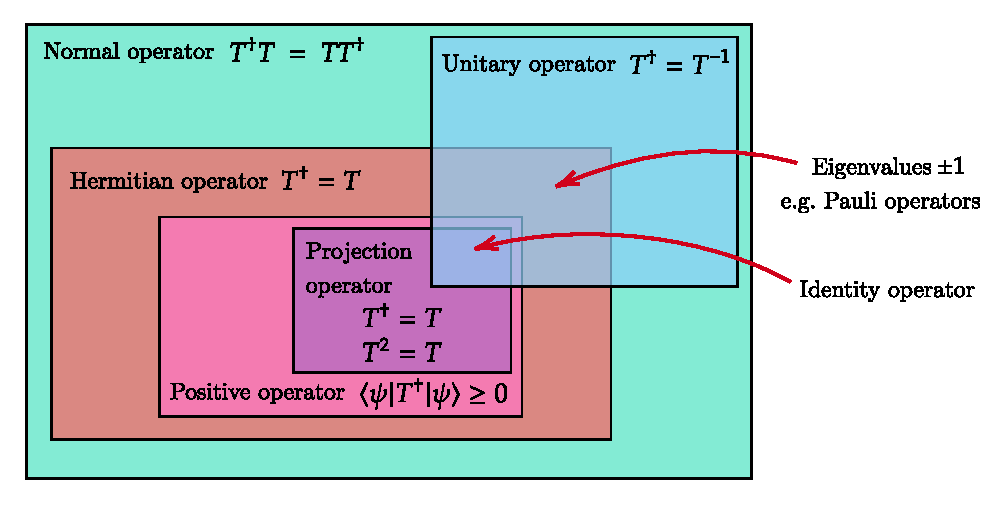
\includegraphics[scale=1]{fig/operator-classification.pdf}
	\caption{Taxonomy of linear operators that possess the spectral decomposition.}
	\label{fig:taxonomy}
\end{figure}

\begin{lemma}\label{}
	Over the field $\C$, positivity implies Hermiticity.\mn{A counterexample over $\R$:
	\begin{align*}
	\mqty(x&y) &\mqty(2&2\\0&0) \mqty(x\\ y) \\ &= x^2 + y^2 + (x+y)^2 \ge 0	
	\end{align*}}
	\begin{align}
		\expval{\op T}{\psi}, \forall\ket{\psi}\in\hilb \implies \op T\dgg = \op T.
	\end{align}
\end{lemma}
\begin{proof}
 	Let $\op T$ be a positive operator. Write $\hat T = \op H + i\op G$, and let $\ket{g_j}$ be normalized eigenvectors of $\op C$ corresponding to eigenvalues $\lambda_j$. For
 	\begin{align}
 		0 \le \expval{\op T}{g_j} = \underbrace{\expval{\op H}{g_j}}_{\textrm{Real}} + i\lambda_j 
 	\end{align}
 	to be true, $\lambda_j$ must vanish for all $j$. Since $\op G$ is Hermitian and all its eigenvalues vanish, it must be the zero operator. Therefore, $ \op T$ is Hermitian.
\end{proof}

\begin{lemma}\label{}
	For any linear operator $\op T$, $\op T\dgg\op T$ and $\op T\op T\dgg$ are positive operators
\end{lemma}
\begin{proof}
	\begin{align}
		\expval{\op T\dgg \op T}{\psi} = (\bra{\psi} \op T\dgg)(\op T\ket{\psi}) = \norm{\op T\ket{\psi}}^2 \ge 0.
	\end{align}
\end{proof}

\begin{lemma}\label{}
    $\op T\dgg \op T = \op\id \iff \op T\op T\dgg = \op\id$ in finite dimensions.
\end{lemma}

\begin{proof}
    Suppose that $\{\ket{e_j}\}$ is an ONB. Since $\op T\dgg\op T=\op\id$, $\ket{f_j} = \op T\ket{e_j}$ also form an ONB. Furthermore,
    \begin{align}
        \ket{f_j} = \op T\ket{e_j} = \op T \op T\dgg \op T\ket{e_j} = \op T\op T\dgg \ket{f_j}.
    \end{align}
    
    to be true for any $j$, it must be the case that $\op T \op T\dgg=\op\id$. The proof in the inverse direction proceeds similarly.

    The proof fails in infinite dimension. Despite the fact that $\{\ket{f_j}\}$ is an orthonormal set of infinite cardinality, there is no guarantee that it spans $\hilb$. For an explicit counterexample, consider the left shift $\op L$ \eqref{eq:left-shift} and the right shift $\op R$ \eqref{eq:right-shift}. They are adjoints of each other (check this!), and it is evident that $\op L\op R =\op\id$, but $\op R\op L\neq \op\id$ because the left shift irrecoverbly kills the first component of any vector.
\end{proof}



	

\newpage

%===============================
%------------------------------
\section{Postulates of quantum theory}
%------------------------------
%===============================

%---------------------------------------------
\subsection{Quantum states and basis measurements}
%---------------------------------------------

\begin{empheq}[box=\fbox]{align}
	\textrm{State} &\longleftrightarrow \textrm{Vector}  \\
	\textrm{Measurement} &\longleftrightarrow \textrm{Projection operator} \\
	\textrm{Dynamics} &\longleftrightarrow \textrm{Unitary operator}  
\end{empheq}


Any ONB gives a {\bf basis measurement}, which defines a probability distribution,
\begin{align}
	p_k &= \abs{\av{e_k|\psi}}^2 = \langle\psi {\color{teal}\overbracket{\dyad{e_k}}^{\op P_k}} \psi \rangle = \expval{\op P_k}{\psi},
\end{align}
$\sum_k \op P_k = \op\id$. For $p_k$ to be a probability, the state must therefore be normalized to 1:
\begin{align}
	\norm{\psi} = \sqrt{\av{\psi|\psi}} = 1.
\end{align}
After the measurement, the state is updated to the basis state $\ket{e_k}$ through the action of the projector,
\begin{align}
	\frac{\op P_k\ket{\psi}}{\sqrt{p_k}} = \frac{\op P_k\ket{\psi}}{\sqrt{\expval{\op P_k}{\psi}}}.
\end{align}
Observe that multiplying a state vector by a complex phase has no effect on any empirical prediction. This can be seen from the following equation.
\begin{align}
	|\mel{\phi}{e^{i\delta}}{\psi}|^2 &= \cancelto{1}{|e^{i\delta}|^2} \abs{\av{\phi|\psi}}^2
\end{align}
This type of phase is commonly referred to as a {\bf global phase} as opposed to a {\bf relative phase}, which, on the other hand, gives rise to interference phenomena, a hallmark of quantum theory.
\begin{align}
	\abs{\bra{\phi}(\ket{\psi_1} + e^{i\delta} \ket{\psi_2})}^2 &= |{\color{maincolor}\overbracket{\color{black}\av{\phi|\psi_1}}^{\psi_1}} + e^{i\delta}{\color{eqcolor}\overbracket{\color{black}\av{\phi|\psi_2}}^{\psi_2}}|^2 \\
	&= \abs{\psi_1}^2 + \abs{\psi_2}^2 + {\color{magenta}\underbracket{2\mathrm{Re}(e^{i\delta}\psi_1^* \psi_2)}_{\textrm{Quantum interference}}}
\end{align}



%---------------------------------------------
\subsection{Case study: qubit}
%---------------------------------------------

A two-level system, or a \emph{qubit}, is any quantum system that can be described by a two-dimensional Hilbert space. We denote the standard ONB as $\{\ket{0},\ket{1}\}$.
\begin{align}
	\ket{\psi} &= \alpha\ket{0} + \beta\ket{1} \\
	&=  ae^{i\gamma}\ket{0} + be^{i\delta}\ket{1} \mnf{Polar form where $a,b,\gamma,\delta$ are real numbers.} \\
	&=e^{i\gamma}\biggl[{\color{maincolor}\underbrace{\cos(\frac{\theta}{2})}_{a}} \ket{0} + e^{i{\color{teal}\tikzmark{a}\varphi}} {\color{eqcolor}\underbrace{\sin(\frac{\theta}{2})}_{b}}\ket{1}\biggr]
\end{align}
\begin{tikzpicture}[remember picture,overlay]
	\draw[<-] 
	([shift={(3pt,6pt)}]a) |- ([shift={(10pt,20pt)}]a) 
	node[anchor=west] {\scriptsize{\color{teal}$\delta-\gamma$}}; 
\end{tikzpicture}
By normalizing the state vector and eliminating the global phase, we have parametrized the state of a qubit by two spherical coordinates $0\le \theta \le \pi$ and $0\le \varphi < 2\pi$.
\begin{figure}[h]
	\centering
	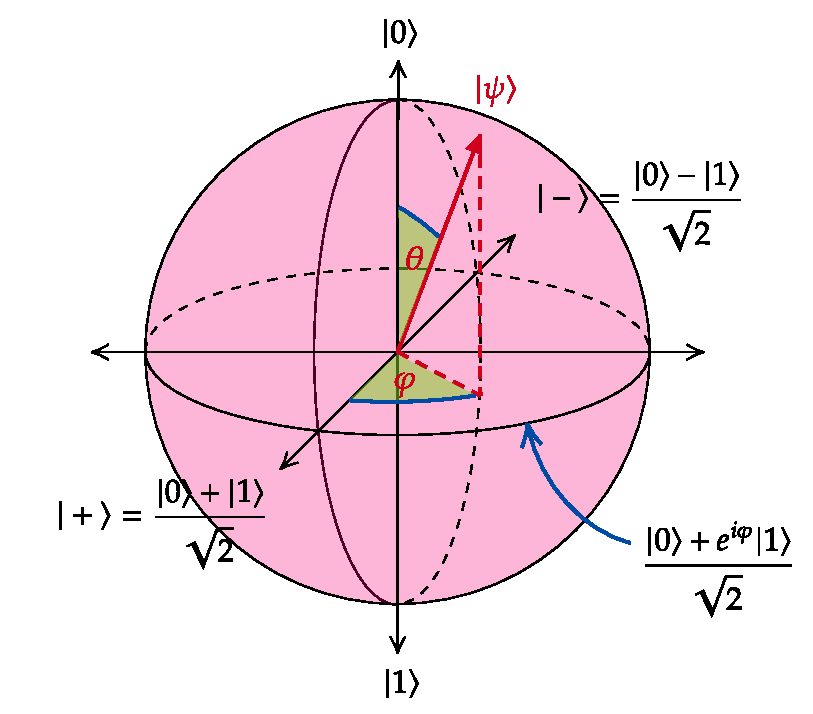
\includegraphics[scale=0.75]{fig/bloch.pdf}
	\caption{Space of qubit states is represented by the Bloch sphere.}
	\label{}
\end{figure}

\noindent Why the one half in $\theta/2$? Look at the operator space,\mn{Given a general state of a two-level system, $\ket{\psi}=\alpha\ket{0}+\beta\ket{1}$, the orthogonal state (up to a phase) can be written as $\ket{\psi^{\perp}}=-\beta^*\ket{0}+\alpha^*\ket{1}$.}
\begin{align}
	\ket{\bf \hat n} &= \cos(\theta/2) \ket{0} + \sin(\theta/2) e^{i\varphi} \ket{1} \\
	\ket{\bf -\hat n} &= -\sin(\theta/2)e^{-i\varphi} \ket{0} + \cos(\theta/2) \ket{1}
\end{align}
\begin{align}
	\dyad{\bf \hat n} &\longleftrightarrow \frac{1}{2} \mqty(1+\cos\theta && \sin\theta\,e^{-i\varphi} \\ \sin\theta\,e^{i\varphi} && 1-\cos\theta)  \mnf{Angel doubling formulae: 
	\begin{align*}
	\sin(\theta) &= 2\sin(\theta/2)\cos(\theta/2), \\
	\cos(\theta) &= \cos^2(\theta/2) - \sin^2(\theta/2) \\ 
	&= 2\cos^2(\theta/2) - 1.	
	\end{align*}} \\
	&= \frac{1}{2}\mqty(1+z & x-iy \\ x+iy & 1-z) \\
	&= \boxed{\frac{\id + \boldsymbol{\hat n \cdot \sigma}}{2}}\, , 
\end{align}
where 
\begin{align}
	\boldsymbol{\sigma} = \mqty(\hat\sigma_x \\ \hat\sigma_y \\ \hat\sigma_z)
\end{align}
is the vector of Pauli matrices
\begin{align}
	\hat\sigma_x = \mqty(0&1\\1&0), &&  \hat\sigma_x = \mqty(0&-i\\i&0), && \hat\sigma_x = \mqty(1&0\\0&-1).
\end{align}
Similarly,\mn{The matrix form can also be obtained from that of $\dyad{\bf \hat n}$ by setting \begin{align*}
		\theta &\leftarrow \pi-\theta, \\
		\varphi &\leftarrow \pi+\varphi. 
\end{align*}}
\begin{align}
	\dyad{\bf -\hat n} &\longleftrightarrow \frac{1}{2} \mqty(1-\cos\theta && -\sin\theta\,e^{-i\varphi} \\ -\sin\theta\,e^{i\varphi} && 1+\cos\theta) = \frac{\id + {(-\boldsymbol{\hat n}) \cdot \boldsymbol\sigma}}{2} 
\end{align}
Spin observable in any direction ${\bf \hat{n}}$
\begin{align}
	\hat\sigma_{\bf \hat n} \equiv \boldsymbol{\hat n\cdot\sigma} = \dyad{\bf \hat n} - \dyad{-\hat {\bf n}} \longleftrightarrow \mqty(\cos\theta && \sin\theta\,e^{-i\varphi} \\ \sin\theta\,e^{i \varphi} && \cos\theta) 
\end{align}
To further investigate the relation between the geometry of the Hilbert space and that of the Euclidean space (inner product $\iff$ geometry), we need to know some properties of Pauli operators.

\vspace{0.5em}
\noindent{\bf Algebraic properties of Pauli operators} 
\begin{enumerate}
	\item $\hat\sigma_j\dgg = \hat\sigma_j$,
	\item $\hat\sigma_j^2 = \id$,
	\item $\hat\sigma_j \hat\sigma_k = i\hat\sigma_l$ where $(j,k,l)$ are cyclic,
	\item $\tr\sigma_j = 0$.
\end{enumerate}
Properties 2 and 3 can be rephrased in terms of the commutator and the anticommutator are
\begin{align}
	[\hat\sigma_j,\hat\sigma_k] = 2i\epsilon_{jkl}\hat\sigma_l, &&
	\{\hat\sigma_j,\hat\sigma_k\} = 2\delta_{jk}\op\id.
\end{align}
Both are encapsulated in the relation
\begin{align}\label{eq:pauli-algebraic}
	\boxed{\hat\sigma_j \hat\sigma_k = \delta_{jk}\op\id + i\epsilon_{jkl}\hat\sigma_l}\, ,
\end{align}
which can be summarized concisely as follows: {\bf Pauli matrices either commute or anticommute}.

\vspace{0.5em}
\noindent 
{\bf Expectation value of Pauli observables.} 
\begin{align}
	\expval{\op\sigma_j}{\bf \hat{n}} &= \tr(\dyad{\bf \hat{n}}\hat\sigma_j) = \tr[\left(\frac{\op\id + \boldsymbol{\hat n \cdot \sigma}}{2}\right)\hat\sigma_j] \\
	&= \frac{1}{2}\tr(\op\sigma_j + \sum_k n_k \hat\sigma_k \hat\sigma_j)
\end{align}
The only term whose trace does not vanish is the identity term from \eqref{eq:pauli-algebraic}. Therefore,
\begin{align}
	\expval{\op\sigma_j}{\bf \hat{n}} &= \frac{1}{2} \sum_k n_k \delta_{jk} \tr \op\id = n_j.
\end{align}
Since a general spin observable is just ${\bf \hat{n}}\cdot \boldsymbol{\sigma}$, the expectation value of spin in $\bf \hat{m}$ direction is ${\bf \hat{n}\cdot\hat{m}}$.
One consequence of this result is that, to determine an unknown state of a two-level system, it is sufficient to find the expectation value of the three Pauli matrices.
\begin{align}
	\mqty(n_x \\ n_y \\ n_z) = \mqty(\av{\hat\sigma_x} \\ \av{\hat\sigma_y} \\ \av{\hat\sigma_z})
\end{align}
This is an example of \emph{quantum state tomography}.

\begin{mybox}[Levi-Civita tensor]
	The Levi-Civita tensor can be used to define the $d$-dimensional totally anti-symmetric vector product. In three dimension,
	\begin{align}
		\epsilon_{jkl} = 
		\begin{cases}
			+1, &(j\;k\;l) \; \textrm{is an \emph{even} permutation} \: (1\; 2\; 3), (2\; 3\; 1), \textrm{or} \; (3\; 1\; 2), \\
			-1, &(j\;k\;l) \; \textrm{is an \emph{odd} permutation} \: (1\; 3\; 2), (2\; 1\; 3), \textrm{or} \; (3\; 2\; 1), \\
			0, &\mathrm{Otherwise}.
		\end{cases}
	\end{align} 
	Here is a few facts about the Levi-Civita tensor. The determinant of a $3\times3$ matrix $M$ can be expressed as the anti-symmetric product of its rows $\det M = \epsilon_{jkl} M_{1j}M_{2k} M_{3l}$. Thus, we have an alternative expression for the cross product:
	\begin{align}
		\vb{A \times B} = \vb{\hat e_j} \epsilon_{jkl} A_k B_l = \det \mqty(\vb{\hat e}_1 & \vb{\hat e}_2 & \vb{\hat e}_3  \\ A_1 & A_2 & A_3 \\ B_1 & B_2 & B_3 ) 
	\end{align}
	A contraction of two Levi-Civita tensors gives an expression involving the Kronecker deltas.
	\begin{align}
		\epsilon_{jkl}\epsilon_{jmn} &= \delta_{km} \delta_{lm} - \delta_{kn} \delta_{lm}, 
		\marginnote{$\delta_{jk}\delta_{jk} = \delta_{jj} = \tr \hat\id_{d\times d} = $ the dimension of the space}\\
		\epsilon_{jkl}\epsilon_{jkm} &= \delta_{kk}\delta_{lm} - \delta_{km} \delta_{lm} = (\dim-1)\delta_{lm} = 2\delta_{lm}
	\end{align}
\end{mybox}

\noindent Now we can compute the inner product in a painless way without needing to use any trigonometric identity.
\begin{align}
	\abs{\ip{\bf \hat n}{\bf \hat m}}^2 &= \frac{1}{4}\tr
	\left[ \left(\id + \boldsymbol{\hat n\cdot\sigma}\right) \left(\id + \boldsymbol{\hat m\cdot\sigma}\right) 
	\right] \\
	&= \frac{1}{4}\tr[ \id +  \underbrace{\boldsymbol{\hat n\cdot\sigma} + \boldsymbol{\hat m\cdot\sigma}}_{\textrm{Traceless}} + (\boldsymbol{\hat n\cdot\sigma})(\boldsymbol{\hat m\cdot\sigma})] \\
	&= \frac{1}{2} + \frac{1}{4}\tr[(\boldsymbol{\hat n\cdot\sigma})(\boldsymbol{\hat m\cdot\sigma})]
\end{align}
What is the trace of $(\boldsymbol{\hat n\cdot\sigma})(\boldsymbol{\hat m\cdot\sigma})$? Use the index notation.
\begin{align}
	(\boldsymbol{\hat n\cdot\sigma})(\boldsymbol{\hat m\cdot\sigma}) &= n_j m_k \hat\sigma_k \hat\sigma_k \\
	&= n_jm_k (\delta_{jk}\id + i\epsilon_{jkl}) \\
	&= n_jm_j\id + i\underbrace{\epsilon_{jkl}n_jm_k}_{({\bf \hat n \times \hat m})_l} \hat\sigma_l \\
	&= ({\bf \hat n \cdot \hat m})\id + \underbrace{({\bf \hat n \times \hat m}) \cdot \boldsymbol{\sigma}}_{\textrm{Traceless}}
\end{align}
To sum up,
\begin{align}
	\boxed{\abs{\ip{\bf \hat n}{\bf \hat m}}^2 = \frac{1+{\bf \hat n \cdot \hat m}}{2}}\, ,
\end{align}  
relating the geometry of the Hilbert space and the Euclidean space. In other words, if the angle between the Euclidean vectors ${\bf \hat n}$ and ${\bf \hat n}$ is $\Theta$, then
\begin{align} 
	\abs{\ip{\bf \hat n}{\bf \hat m}}^2 = \frac{1+\cos\Theta}{2} = \cos^2\left(\frac{\Theta}{2}\right).
\end{align}                            
Notice the angle doubling effect again.  


%---------------------------------------------
\subsection{Quantum dynamics}
%---------------------------------------------

$\dv{t}$ acts linearly on the state $\ket{\psi}$, so we should be able to represent it by a linear operator $\hat{G}$. What kind of operator $\hat{G}$ is for the time evolution to preserve the inner product?
\begin{align}
	0=\dv{t} \av{\psi|\psi} &= \left(\dv{t} \bra\psi\right) \ket\psi + \bra\psi \left(\dv{t}\ket\psi\right) \\
	&= \ev{\hat G\dgg}{\psi} + \ev{\hat G}{\psi} \\
	&= \ev{(\hat G\dgg + \hat G)}{\psi} 
\end{align}
implying that $\op G$ is anti-Hermitian, $\hat G\dgg = -\hat G$. The dimension of $\op G$ should be that of $[\textrm{time}]^{-1}$. Physicists set it to be $\op G = \op H/i\hbar$, where $\op H$ is a Hermitian \emph{Hamiltonian operator}.\mn{This ``derivation" of the Schr\"odinger equation contains no physics, so we cannot expect it to give the value of the constant $\hbar$.}

\begin{definition}[\bf Schr\"odinger equation]\leavevmode
	\begin{align}
		i\hbar \dv{t} \ket{\psi(t)} = \op H \ket{\psi(t)}
	\end{align}
\end{definition}
The Schr\"odinger equation relates an instantaneous change in the state vector to the Hamiltonian operator. A more ``global", operator-version of Schr\"odinger equation is also illuminating when $\op H$ does not depend on time,\mn{This requires in particular that $\op H$ at different times commute with itself. Otherwise, we need to use \href{http://scipp.ucsc.edu/~haber/ph215/TimeOrderedExp.pdf}{time-ordered exponentials}.}
\begin{align}
	i\hbar \dv{t} \op U(t) \ket{\psi(0)} &= \op H \op U(t) \ket{\psi(0)} \\
	i\hbar \dv{U(t)}{t} &= \op H \op U(t) \\
	\frac{\textrm{d}\op U(t)}{\op U(t)} &= -\frac{i}{\hbar} \op H \textrm{d}t \mnf{The meaning of this strange-looking matrix different equation is that we have differential equations for the eigenvalues in the basis in which $\op U$ is diagonal.} \\
	\Aboxed{\op U(t) &= e^{-i\op Ht/\hbar}}\, .
\end{align}

%---------------------------------------------
\subsection{*Looking ahead}
%---------------------------------------------

The Schr\"odinger equation only applies to a closed system, but ``closed" here does not mean the absence of an energy or mass exchange with the surroundings; it means the absence of \emph{communication} with the outside world. Thus, it is more accurate to say that quantum phenomena happen to systems that are \emph{informationally isolated}. For an \emph{open quantum system}, the quantum formalism has to be modified as follows.

\begin{empheq}[box=\fbox]{align}
	\textrm{State} &\longleftrightarrow \textrm{Positive operator}  \\
	\textrm{Measurement} &\longleftrightarrow \textrm{Positive operator} \\
	\textrm{Dynamics} &\longleftrightarrow \textrm{Completely positive map}\mnf{The meaning of complete positivity is outside the scope of this lecture.}  
\end{empheq}
Therefore, the notion of information is already baked into the formalism of quantum theory at a fundamental level.
In my opinion, Rolf Landauer's slogan ``information is physical" is at its most profound in the quantum world.




	

\newpage

%===============================
%------------------------------
\section{Quantum Information and Ebits (Entanglement Bits)}
%------------------------------
%===============================

%---------------------------------------------
\subsection{Tensor product}
%---------------------------------------------

The quantum state of a joint system $AB$ lives in the tensor product space $\hilb_A\otimes \hilb_B$. The tensor product space can be defined without relying on specific bases on $\hilb_A$ and $\hilb_B$, but for the sake of simplicity, we will define the tensor product  via ONBs.

Suppose that $\{\ket{e_j}\}_j$ and $\{\ket{f_k}\}_k$ are ONBs for $\hilb_A$ and $\hilb_B$ respectively. (Their dimensions may not be the same.) $\hilb_A\otimes \hilb_B$ is simply the span (formal linear combinations) of elements in the Cartesian product $\{\ket{e_j}\}_j \times \{\ket{f_k}\}_k$, denoting the elements by $\ket{e_j}\otimes \ket{f_k}$.

A vector in $\hilb_A\otimes\hilb_B$ is said to be a {\bf product state} if it can be written as a simple product $\ket{\psi}\otimes\ket{\phi}$ of some $\ket{\psi}\in\hilb_A$ and $\ket{\phi}\in\hilb_B$. Otherwise, a vector is said to represent an {\bf entangled state}.
If needed, subscripts may be added to indicate which vector belongs to which Hilbert space, for example, $\ket{\psi}_A \otimes \ket{\phi}_B$. 
It is common to omit the tensor product symbol $\otimes$ and write a product state simply as $\ket{\psi}\ket{\phi}$, or even $\ket{\psi\phi}$ when no confusion may arise. The latter is extremely common when the qubit basis states are labeled by binary numbers, for example $\ket{00} = \ket{0}\otimes\ket{1}, \ket{01}=\ket{0}\otimes\ket{1}$, and so on.)
 
\vspace{0.5em}
\noindent {\bf Scalar multiplication}
\begin{align}
	\lambda(\ket{\psi}\otimes\ket{\phi}) &= 
	(\lambda\ket{\psi})\otimes\ket{\phi} =
	\lambda(\ket{\psi}\otimes(\lambda\ket{\phi}) 
\end{align}
\vspace{0.5em}
\noindent {\bf Vector addition}
\begin{align}
	(\ket{\psi_1} + \ket{\psi_2}) \otimes \ket{\phi} &= \ket{\psi_1} \otimes \ket{\phi} +  \ket{\psi_2} \otimes \ket{\phi} \\
\ket{\psi}\otimes(\ket{\phi_1} + \ket{\phi_2}) &= \ket{\psi}\otimes \ket{\phi_1}  + \ket{\psi}\otimes  \ket{\phi_2}	
\end{align}
Compare these to the rules \ref{direct-sum-add} and \ref{direct-sum-scalar} for the direct product (which is equivalent to the direct sum) of vector spaces.

Linear combinations of product vectors with no common factor (entangled states) are genuinely new objects in $\hilb_A \otimes \hilb_B$.

\vspace{0.5em}
\noindent {\bf Inner product.}
\begin{align}
	(\bra{\eta}\otimes\bra{\xi}) (\ket{\psi}\otimes\ket{\phi}) 
	= \av{\eta|\psi}\av{\xi|\phi}
\end{align}

\vspace{0.5em}
\noindent {\bf Partial inner product.}
\begin{align}
	{}_A\bra{\eta} (\ket{\psi}_A\otimes\ket{\phi}_B) 
	= \av{\eta|\psi}\ket{\phi}_B
\end{align}

\vspace{0.5em}
\noindent {\bf Linear operators.}
\begin{align}
	\op A\otimes \op B (\ket{\psi}\otimes\ket{\phi}) &= 
		(\op A\ket{\psi}) \otimes (\op B\ket{\phi}) \\
	(\op A \otimes \op B)(\op C\otimes \op D) &= (\op A \op C)\otimes (\op B \op D)
\end{align}
Thus, the trace factorizes.
\begin{align}
	\tr(\op A\otimes \op B) &= \sum_{jk} \bra{e_j} \bra{f_k} \op A\otimes \op B \ket{e_j}\ket{f_k} \\
	&= \sum_{jk} \mel{e_j}{\op A}{e_j} \mel{f_k}{\op B}{f_k} \\
	&= \tr(\op A) \otimes \tr(\op B)
\end{align}
\emph{Local operations} always commute.
\begin{align}
	[\op A\otimes \op\id, \op\id\otimes \op B] = \op A \otimes \op B - \op A \otimes \op B = 0
\end{align}
If one wants to represent a tensor product operator in a matrix form, one needs to fix the ordering of the bases of $\hilb_A \otimes \hilb_B$.\mn{By doing this, we are representing higher-rank tensors as a two-tensor (a matrix), and there is no canonical way to do it. It is more natural to represent them as they are, using quantum circuit diagrams or tensor diagrams \cite{coecke2009}.} When the lexicographic ordering is chosen, the matrix form has the form of the Kronecker product, which only shown here for the 2-by-2 case:
\begin{align}
	\op A \op B \longleftrightarrow \left(\begin{array}{c;{2pt/2pt}c}
		A_{00}B & A_{01}B \\ \hdashline[2pt/2pt]
		A_{10}B & A_{11}B 
	\end{array}\right).
\end{align}

\begin{mybox}
The concept of tensor product is typically introduced to studentss in a highly unintuitive setting of quantum theory, and as a result, the idea may appear alien at first. However, the tensor product is already present in ordinary probability theory as a self-evident means of combining the probabilities of two independent random variables.
\begin{align}
	\mqty(p \\ 1-p) \otimes \mqty(q\\1-q) = \mqty(pq \\ p(1-q) \\ (1-p)q \\ (1-p)(1-q))
\end{align}
In ordinary probability theory, a state that cannot be written as a product state $\ket{p}\otimes\ket{q}$ is a {\bf correlated state}. Entanglement is a form of correlation, but we will see in Section \ref{sec:A01} that it can be stronger than any classical correlation.
\end{mybox}

%---------------------------------------------
\subsection{Communication using entanglement}
%---------------------------------------------

The four {\bf Bell states} are defined to be
\begin{align}
	\ket{\Phi_{\pm}} &\equiv \frac{\ket{00}\pm\ket{11}}{\sqrt{2}}, \\
	\ket{\Psi_{\pm}} &\equiv 
	\frac{\ket{01}\pm\ket{10}}{\sqrt{2}}.
\end{align}
It is straightforward to verify that they form an ONB. Therefore, they constitute a basis measurement called the {\bf Bell measurement}.\mn{The Bell measurement is a prime example of a basis measurement that is not conventionally associated to any observable (i.e. a Hermitian operator).}
Alternatively, they can be arranged in a convenient form, 
\begin{align}\label{eq:steering}
	\ket{\Omega_{{\color{magenta}\tikzmark{a}a}{\color{eqcolor}\tikzmark{b}b}}} \equiv \op\id\otimes \op X^a\op Z^b \ket{\Omega},
\end{align}



\begin{tikzpicture}[remember picture,overlay]
	\draw[<-] 
	([shift={(2pt,-2pt)}]a) |- ([shift={(-10pt,-10pt)}]a) 
	node[anchor=east] {\scriptsize{\color{magenta}Parity bit}}; 
	\draw[<-] 
	([shift={(2pt,-2pt)}]b) |- ([shift={(14pt,-10pt)}]b) 
	node[anchor=west] {\scriptsize{\color{eqcolor}Phase bit}}; 
\end{tikzpicture}


\noindent obtained from  $\ket{\Omega}\equiv \ket{\Phi_+}$ via a local Pauli operation. In particular,
\begin{align}
	\ket{\Omega_{00}} &= \op\id\otimes\op\id\ket{\Omega} = \frac{\ket{00}+\ket{11}}{\sqrt{2}}, \\
	\ket{\Omega_{01}} &= \op\id\otimes\op Z\ket{\Omega}= \frac{\ket{00}-\ket{11}}{\sqrt{2}}, \\
	\ket{\Omega_{10}} &= \op\id\otimes\op X\ket{\Omega}= \frac{\ket{01}+\ket{10}}{\sqrt{2}}, \\
	\ket{\Omega_{11}} &= \op\id\otimes\op X \op Z\ket{\Omega}= \frac{\ket{01}-\ket{10}}{\sqrt{2}}.
\end{align}

\begin{lemma}\label{}
	For any linear operator $\op T$,
	\begin{align}
		\op\id\otimes \op T\ket{\Omega} = \op T^T \otimes \op\id \ket{\Omega},
	\end{align}
	where $^T$ denotes the matrix transposition. In particular, we have that
	\begin{align}
		\ket{\Omega_{11}} = \op\id\otimes \op X\op Z\ket{\Omega} = \op Z\op X \otimes \op\id \ket{\Omega}.
	\end{align}
\end{lemma}


In the followings, we suppress the tensor product symbol when writing two-body Pauli operators: $\op \sigma_j \op \sigma_k = \op \sigma_j \otimes \op \sigma_k$.
Since
\begin{align}
	\op Z\op Z\ket{x_1}\ket{x_2}=(-1)^{x_1\oplus x_2}\ket{x_1}\ket{x_2}, && 
	\op X\op X\ket{x_1x_2}=(-1)^{x_1\oplus x_2}\ket{x_1\oplus 1}\ket{x_2\oplus 1},
\end{align}
we can see that $\op Z \op Z$ measures the parity bit and $\op X \op X$ measures the phase bit,
\begin{align}
	\op Z\op Z \ket{\Omega_{ab}} &= (-1)^a \ket{\Omega_{ab}}, \\
	\op X\op X \ket{\Omega_{ab}} &= (-1)^b \ket{\Omega_{ab}}.
\end{align}
For $\op Y \op Y$, note that
\begin{align}
	-\op Y \op Y =  (\op Z \op Z)(\op X \op X).
\end{align}
Therefore
\begin{align}
		-\op Y\op Y \ket{\Omega_{ab}} &= (-1)^{a\oplus b} \ket{\Omega_{ab}}.
\end{align}

Special attention should be paid to the {\bf singlet state} $\ket{\Psi_-} = (\ket{01}-\ket{10})/\sqrt{2}$ with the property that simultaneous spin measurements on the two qubits in the same direction are always \emph{anti-correlated}. In particular, the state can be written as
\begin{align}
	\frac{\ket{\hat{\vb n}}\ket{-\hat{\vb n}} - \ket{-\hat{\vb n}}\ket{\hat{\vb n}}}{\sqrt 2}
\end{align}
The singlet state can be prepared, for instance, via the process of spontaneous parametric down-conversion (SPDC) that produces a photon pair with opposite polarizations.



\begin{example}[\bf Superdense coding]\leavevmode
	
	Equation \eqref{eq:steering} implies that if Alice and Bob possess an entangled pair $\ket{\Omega}$, Alice can communicate two bits of information (the parity bit and the phase bit) to Bob by choosing to perform a Pauli operation on her side and send the qubit to Bob. In the form of \emph{Bennett's law}, we state that
	\begin{align}\label{eq:superdense}
		\textrm{1 ebit + 1 qubit} \succ \textrm{2 bits},
	\end{align} 
	where $\succ$ means ``can perform a task in place of".
\end{example}

\begin{example}[\bf Teleportation]\leavevmode
	
	The ``converse" to \eqref{eq:superdense},
		\begin{align}\label{eq:teleport}
		\textrm{1 ebit + 2 bits} \succ \textrm{1 qubit},
	\end{align} 
	is \emph{quantum teleportation}. Alice and Bob again begins the protocol with a pre-shared entanglement $\ket{\Omega}$, but now Alice has an unknown state $\ket{\psi}$ that she wants to send to Bob. Rather than sending the qubit directly (which would need a high-fidelity quantum channel, for example), what Alice can do is performing the Bell measurement on her unknown state and one half of the Bell pair. Remarkably, depending on the two-bit outcome $ab$ that Alice obtained, the post-measurement state on Bob's side becomes
	\begin{align}
		\ket{\psi'} = \op X^b \op Z^a \ket{\psi},
	\end{align}
which is not exactly the state $\ket{\psi}$ that Alice wants to send, but the extra Pauli operators can be corrected away with the information of the bits $ab$ that Alice can tell Bob by calling him on a phone, for example.
\end{example}
	
Proofs of the teleportation protocol found in textbooks are often quite long and involve some unintuitive steps. The following short proof is inspired from the tensor diagrammatic proof \cite{coecke2009}.
Let the subscripts $A,B$, and $C$ denote the Hilbert space of Alice's unknown qubit state, the Hilbert space of one half of the Bell pair that Alice holds, and the Hilbert space of the other half of the Bell pair that Bob holds, respectively.  
	\begin{align}
		{}_{AB}\bra{\Omega_{ab}} \left(\ket{\psi}_A \ket{\Omega_{00}}_{BC}\right)
		&= \frac{1}{2} \left[\sum_j \bra{j}_A \bra{j}_B(\op Z^a \op X^b)_A\dgg \otimes \op \id_B\right] \ket{\psi}_A \sum_k \ket{k}_B \ket{k}_C \\
		&= \frac{1}{2} \sum_{jk} \bra{j}_A\underbrace{\op X^b \op Z^a \ket{\psi}_A}_{\ket{\psi'}} \underbrace{\bra{j}_B\ket{k}_B}_{\delta_{jk}} \ket{k}_C\\
		&= \frac{1}{2} \sum_j \braket{j}{\psi'} \ket{j}_C\\
		&= \frac{1}{2} \ket{\psi'}_C
	\end{align}
	The subnormalization factor 1/2 tells us that the outcome probability for the Bell measurement is uniform.


%---------------------------------------------
\subsection{EPR argument}
%---------------------------------------------

A philosophical troubling aspect of quantum theory is that one cannot in general think of an act of measuring as revealing a pre-existing value of the measured property. When the system is in an eigenstate of an observable $\hat A$ with an eigenvalue $\lambda$, subsequent measurements of $\hat A$
do not alter the state, hence there is a tendency to think of the value $\lambda$ as pre-existed. Einstein, Padolsky, and Rosen (EPR) devised a clever argument using quantum correlation and the principle of relativity to argue that values of incompatible (non-commuting) observables can simultaneously pre-exist.
\begin{figure}[h]
	\centering
	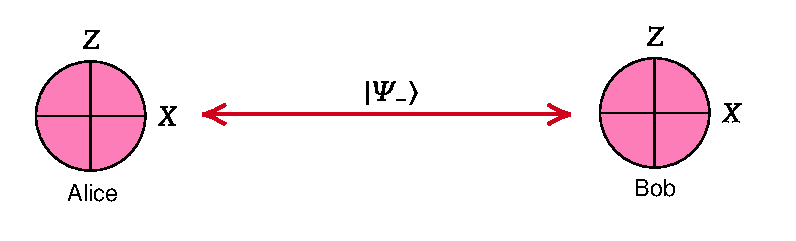
\includegraphics[scale=0.75]{fig/epr-measurement-setting}
	\caption{Measurement settings in the EPR argument.}
	\label{fig:epr-setting}
\end{figure}

The singlet state $\ket{\Omega_{11}}$ is an eigenstate shared by $\op Z\op Z$ and $\op X\op X$ with both eigenvalues -1. (Verify that they commute.) Now, while Alice cannot make a local Z and X measurements at the same time, if she chooses to measure one, say $\op Z_A$ and find the value $z_A = \pm 1$, then the spin of Bob's particle would need to have the opposite value to satisfy $z_A z_B =-1$. Since the spins are anti-correlated in every direction in the singlet stat, the same conclusion follows if Alice were to measure $\op X_A$. But, EPR argued, the act of measurement by Alice over here cannot effect the state of Bob's particle over there. Thus, the fact that Alice could have chosen to measure either observable and inferred $z_B$ or $x_B$ without disturbing Bob's particle means that those values already existed before the measurement.

\begin{align*}
	\left(\parbox{8em}{\centering {\bf Entanglement} \\ Anti-correlation \\ in the singlet state}\right)
	+ \left(\parbox{8em}{\centering {\bf Relativity} \\ The choice of measurement on A cannot have an influence on B}\right)
	\implies 
	\left(\parbox{8em}{\centering {\bf Quantum theory is incomplete}}\right)
\end{align*}

\noindent The EPR correlation in the $Z$ and $X$ measurement outcomes can be explained by classical hidden variables, in particular, Spekkens' toy theory \cite{spekkens2007}. See also \cite{wood2015} for diagrams similar to Figures \ref{fig:epr-setting} and \ref{fig:chsh-setting}.

%---------------------------------------------
\subsection{CHSH inequality}\label{sec:chsh}
%---------------------------------------------

The hope that quantum theory can be completed with \emph{hidden variables} that behave entirely classically is dashed by an experimental violation of the CHSH inequality.\mn{Named after John Clauser, Michael Horne, Abner Shimony, and Richard Hol, the inequality is formulated to be more suitable for experimental tests, an improvement over Bell's inequality.} Here we present a derivation of the CHSH inequality in the setting of a communication game, called a \emph{nonlocal game} in this context \cite{bell-nonlocality-review}.

Consider a communication game involving two players, Alice and Bob. In this cooperative game, Alice and Bob initially have the opportunity to consult and share their strategies before separating and traveling to two distant referees. The players are allowed to communicate in advance, but once the game begins, they are unable to communicate due to the restriction imposed by the speed of light.

\vspace{0.5em}
\noindent {\bf Game structure.}
At the referee stations, two binary questions are randomly chosen, denoted by $x\in\{0,1\}$ for Alice's question and $y\in\{0,1\}$ for Bob's question. Alice and Bob must give answers immediately, represented by variables $a\in\{0,1\}$ and $b\in\{0,1\}$, respectively. Because of the random choices, neither player knows the question in advance, and they cannot communicate the questions they received fast enough to change their answers. The referees then record the answers and later compare notes.

\vspace{0.5em}
\noindent {\bf Winning Condition.}
The goal for Alice and Bob to win the game is for the logical AND of their answers $a\wedge b$ to be equal to the product  of the choices of the questions $xy$. Here, $a\wedge b$ represents whether the answers agree (0) or disagree (1). In other words, they win if the following condition is satisfied:
\begin{align}
	xy = a\wedge b.
\end{align}
The only instance where Alice and Bob's answers must disagree is when $x=y=1$, see Figure \ref{fig:chsh}. 
\begin{marginfigure}
	\centering
	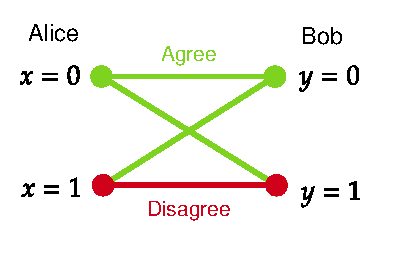
\includegraphics[scale=0.75]{fig/chsh.pdf}
	\caption{Diagram illustrating the rule of the nonlocal game.}
	\label{fig:chsh}
\end{marginfigure}
The agreement-disagreement relationship between the questions and answers forms a \emph{frustration graph}. It becomes evident that it is impossible to assign simultaneous edge values ($a$ and $b$) to satisfy the winning condition. In the case of a deterministic strategy where Alice and Bob always answer yes or no, the game can be won with a probability of 3/4. Remarkably, this represents the best achievable winning probability for Alice and Bob. (The winning probability for mixed strategies is at most equal to that of deterministic strategies.)
This bound on the winning probability
\begin{align}
	\Pr_{\substack{\textrm{win}\\ \textrm{classical}}} \le \frac{3}{4}.
\end{align}
is one form of the CHSH inequality; it signifies the limit of any classical local hidden variable theory.
\begin{align*}
	\left(\parbox{5.5em}{\centering {\bf Classical correlation} }\right)
	+ \left(\parbox{8em}{\centering {\bf Relativity} \\ The choice of measurement on A cannot have an influence on B}\right)
	\implies 
	\left(\parbox{8em}{\centering {\bf CHSH inequality}}\right)
\end{align*}

Now we show that if Alice and Bob have shared the singlet state beforehand, they can win the game with a probability greater than what is permissible by the CHSH bound.
\begin{figure}[h]
	\centering
	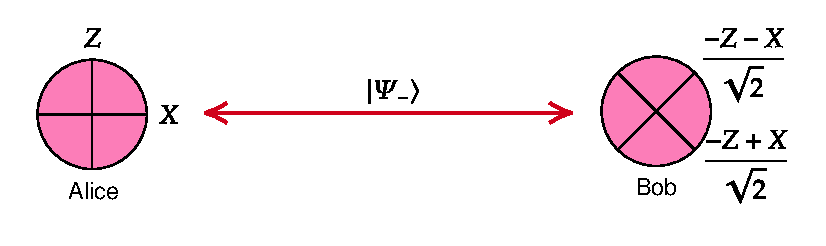
\includegraphics[scale=0.75]{fig/chsh-measurement-setting}
	\caption{Measurement settings that leads to a violation of the CHSH inequality given that Alice and Bob pre-shared the singlet state.}
	\label{fig:chsh-setting}
\end{figure}
\begin{align}
	\Pr_{\textrm{win}} &= \frac{1}{4}(p_{00}^{(+)} + p_{01}^{(+)} + p_{10}^{(+)} + p_{11}^{(-)}) \\
	&= \frac{1}{4}\av{\op P_{00}^{(+)} + \op P_{01}^{(+)} + \op P_{10}^{(+)} + \op P_{11}^{(-)}}
\end{align}
Solve for $\op P^{(\pm)}$ in terms of the observables.
\begin{align}
	\begin{cases}
		\op P^{(+)} + \op P^{(-)} &= \op \id, \\
		 \op P^{(+)} - \op P^{(-)} &= \op \sigma_{xy},
	\end{cases}
	\implies \op P^{(\pm)} = \frac{\op\id + \op\sigma_{xy}}{2}
\end{align}
Thus,
\begin{align}
	\Pr_{\textrm{win}} &= 
	\frac{1}{2} + \frac{1}{8}\av{\op\sigma_{00} + \op\sigma_{01} + \op\sigma_{10}  - \op\sigma_{11}}. 
\end{align}
Specialize to the measurement angles given in...
\begin{align}
\Pr_{\textrm{win}} &=   \frac{1}{2} + 
	\frac{1}{8}\av{\op Z\otimes \frac{-\op Z + \op X}{\sqrt 2} 
	+ \op Z\otimes \frac{-\op Z - \op X}{\sqrt 2}
	+ \op X\otimes \frac{-\op Z + \op X}{\sqrt 2}
	- \op X\otimes \frac{-\op Z - \op X}{\sqrt 2}} \\
	&=  \frac{1}{2} + 
	\frac{1}{8\sqrt 2} \av{\op Z\op Z + \op X \op X} = \frac{1}{2} + \frac{\sqrt 2}{4} \approx 85\% >
	\frac{3}{4} \ge \Pr_{\substack{\textrm{win}\\ \textrm{classical}}},
\end{align}
where the expectation value is taken with respect to the singlet state.

The original form of the CHSH inequality, $S_{\textrm{classical}} \le 2$, is phrased in terms of expectation values, or two-point correlation functions,
\begin{align}
	S = \abs{\av{\op \sigma_{00}} + \av{\op \sigma_{01}} + \av{\op \sigma_{10}} - \av{\op \sigma_{11}}}.
\end{align}
The maximum violation allowed by quantum theory is $S = 2\sqrt{2}$, which is what we achieved in the computation above, called the \emph{Tsirelson bound}. The winning probability of 1 corresponds to the value $S=4$, which is achievable in non-quantum theories that, surprisingly enough, still do not violate special relativity (called \emph{non-signaling theories}) \cite{pr-box}. However, there can be some highly unlikely consequences in a universe in which such  \emph{super-quantum} theory is obeyed such as trivial communication complexity \cite{vandam2012}.


	
	
\newpage

\appendix

\section{Linear Algebra}\label{sec:A01}

%---------------------------------------------
\subsection{Vector space, basis, and dimensionality}
%---------------------------------------------

To define vector space axiomatically, it is convenient to define an abelian group first.

\begin{definition}
	A {\bf group} $G$ is a set closed under an associative binary operation $\cdot$ (\emph{group multiplication}) satisfying the following properties.
	\begin{enumerate}
		\item There exists an {\bf identity} element $e$ such that $e\cdot g = g\cdot e = g$ for every element $g\in G$.
		\item For every $g\in G$, there exists an {\bf inverse} denoted by $g^{-1}$ such that $g\cdot g^{-1} = g^{-1}\cdot g = e$. 
	\end{enumerate}
\end{definition}
\noindent We often omit the symbol $\cdot$ and simply write a product $g\cdot h$ as $gh$.
A group in which the order of multiplication doesn't matter ($gh=hg$) is called a {\bf commutative} group or an {\bf abelian} group.
\begin{example}
	$(\Z,+)$ (The group of integers with addition as group multiplication) is an abelian group with 0 as the identity and $-a$ as the inverse of $a$.
\end{example}
%\begin{example}
%	$(\Z_+,+)$ (The group of non-negative integers) is {\bf not} a group, since any nonzero element has no inverse.
%\end{example}
\begin{example}
	$(\Z,-)$ (The group of integer with subtraction as group multiplication) is {\bf not} a group, since subtraction is not associative ($a-(b-c) \neq (a-b)-c$).
\end{example}
{\color{red}
\begin{example}
	$(\C/\{0\},\times)$ (The group of complex numbers excluding zero with multiplication) is an abelian group with 1 as the identity and $1/a$ as the inverse of $a$.
\end{example}
}
\begin{example}
	$(\{\pm 1,\pm i\},\times)$ is an abelian group with 1 as the identity. $-1$ is its own inverse, and $\pm i$ is an inverse of each other.
\end{example}
\begin{example}
	$(\mathrm{GL}(n),\times)$ (The group of invertible matrices with matrix multiplication) is a non-abelian group with the identity matrix $\id$ as the identity and the matrix inverse $A^{-1}$ as the inverse.
\end{example}
\begin{example}[\bf Quantum information example]\leavevmode
	\noindent $(\{\pm \id, \pm iX, \pm iY, \pm iZ\},\times)$, where
	\begin{align}\label{def:pauli}
		X=\mqty(0&1\\ 1&0), && Y=\mqty(0&-i\\ i&0), &&Z=\mqty(1&0\\0&-1)
	\end{align}
	are \emph{Pauli matrices}, forms a non-abelian group with $\id$ as the identity and $\pm iX$ is an inverse of each other, for example.
\end{example}

Armed with the definition of an abelian group, we now proceed to define a vector space over the number field $K=\R$ (reals) or $\C$ (complex numbers).
\begin{definition}
	A {\bf vector space} $V$ over $K$ is a set closed under the following  operations.
	\begin{enumerate}
		\item {\bf Vector addition:} $u+v$, where $u,v\in V$,
		\item {\bf Scalar multiplication:} $a u$, where $a\in K$ and $u\in V$,
	\end{enumerate}	 
	such that $(V,+)$ is an abelian group, and 
	\begin{align}
		1u &= u, \\
		a(u+v) &= a u + a v, \\
		(a +b) u &= a u + b u, \\
		(ab) u &= a(b u),	
	\end{align}
	where $u,v\in V$ and $a,b\in K$
\end{definition}

The three-dimensional Euclidean space $\R^3$ is a prototypical example of a vector space over $\R$. As a set, $\R^3$ contains infinitely many vectors, but a finite representative set $\{\bf \hat{x},\hat{y},\hat{z}\}$, called a \emph{basis}, is sufficient to represent any vector in $\R^3$. To define a basis, we first define the notion of a span.

\begin{definition}
	Given a set $S=\{u_1,u_2,\dots,u_n\} \subset V$ of a finite number of vectors, $\mathrm{span}\,S$ is the set of all linear combination (L.C.) of these vectors
	\begin{align}
		a_1u_1 + a_2u_2 + \cdots + a_nu_n, && \forall a_j \in K.
	\end{align} 
\end{definition}

\noindent A vector space $V$ is said to be {\bf finite dimensional} if it is spanned by some finite set of vectors in $V$. Otherwise, it is {\bf infinite dimensional}.

\begin{definition}
	A set $S=\{u_1,u_2,\dots,u_n\} \subset V$ is {\bf linearly independent (L.I.)} if the equation
	\begin{align}
		a_1u_1 + a_2u_2 + \cdots + a_nu_n = 0
	\end{align}
	implies that $a_j = 0$ for all $j=1,\dots,n$. 
\end{definition}
\noindent In other words, linear independence means that no vector in $S$ can be written as a non-trivial L.C. of other vectors in $S$. Otherwise, if $a_1\neq 0$, for instance, then
\begin{align}
	u_1 = -(a_2 u_2 + \cdots + a_n u_n)/a_1.
\end{align}

%\begin{definition}
%	$S \subseteq V$ {\bf spans} $V$ if every vector in $V$ can be written as a linear combination of vectors in $S$.
%\end{definition}

\begin{definition}
	$S\subset V$ is a {\bf basis} for $V$ if it is L.I. and spans $V$.
\end{definition}
\noindent The size of $S$ is an invariant of a vector space called the {\bf dimension}, denoted by $\dim V$. The dimension is the minimum numbers of vectors that spans $V$. For any nontrivial (not $\{0\}$) vector space, there are infinitely many choices of bases.

\begin{example}
	The field $K$ itself is a one-dimensional vector space over $K$.	
\end{example}
\begin{example}
	$K^n$ is an $n$-dimensional vector space over $K$, with the standard basis $\{u_j\}_{j=1,\dots,n}$, where $u_j$ is a vector with 1 at the $j$th entry and 0 elsewhere. 
	
	\noindent In the two-dimensional case, the followings are equivalent fot a set $S = \{(a_1,a_2), (b_1,b_2)\}$.
	\begin{itemize}
		\item $S$ is L.I.
		\item $S$ spans $K^2$.
		\item The determinant $\mqty|a_1&b_1\\a_2&b_2|=a_1b_2 - a_2b_1 \neq 0$.
	\end{itemize}
\end{example}
\begin{example}
	The set of $n\times m$ $K$-valued matrices is an $n\times m$-dimensional vector space with the basis $\{E_{jk}\}_{j=1,\dots,n}^{k=1,\dots,m}$, where $E_{jk}$ is a matrix with 1 at the $jk$th entry and 0 elsewhere. 
\end{example}
%\begin{example}[\bf Quantum computing example]
%	The complex span of $\{\id,X,Y,Z\}$ where $X,Y,Z$ are the Pauli matrices \eqref{def:pauli}. coincides with the set of all complex $2\times 2$ matrices, while the real span of $\{\id,X,Y,Z\}$ coincides with the set of all Hermitian $2\times 2$ matrices.
%\end{example}
\begin{example}
	Polynomials over an indeterminate $x$ form an infinite-dimensional vector space. Restricting to $n$-degree polynomials gives an $(n+1)$-dimensional vector space with a basis $\{1,x,x^2,\dots,x^n\}$.
\end{example}
\begin{example}
	The set of solutions of a linear, $k$th-order differential equation, for example, $$f''+f'+f=0$$ for $k=2$, forms a vector space of dimension $k$.
\end{example}

By choosing a basis, every vector in a finite-dimensional vector space can be specified by its {\bf components} $v_j$ defined as.
\begin{align}
	v = \sum_j v_j u_j,
\end{align}
which is typically stacked into a column vector
\begin{align}
	v \leftrightarrow \mqty(v_1 \\ v_2 \\ \vdots \\ v_n).
\end{align}
The arrow $\leftrightarrow$ is there to remind us that the components constitute only a \emph{representation} of the vector. The vector itself is a geometric object (visualized as an arrow, for example) that exists independent of the choice of basis, whereas the components change when we perform a \emph{change of basis}. (More on that later.)

A subset $S \subset V$ of a vector space that is also a vector space is called a {\bf subspace}.
A vector space $U$ is said to be a {\bf direct sum} $V\oplus W$ if every $u\in U$ can be decomposed uniquely as a sum of $v\in V$ and $w\in W$.
Equivalently, any $u\in U$ can be specified by a unique pair $(v,w)\in V\times W$ such that\mn{Hence for vector spaces, the direct sum and the direct product are the same. Compare properties \ref{direct-sum-add} and \ref{direct-sum-scalar} to the algebraic rules for the tensor product.}
\begin{align}
	(v_1,w_1) + (v_2,w_2) &= (v_1+v_2,w_1+w_2), \label{direct-sum-add}\\
	a(v,w) &= (av,aw). \label{direct-sum-scalar}
\end{align}


%---------------------------------------------
\subsection{Linear maps, eigenvalues, and eigenvectors}
%---------------------------------------------

Morphisms that preserve the structure of vector spaces are linear maps.
\begin{definition}
	Given a map $T:U\to V$,
	$T$ is said to be a {\bf linear map} if
	\begin{align}
		T(au + bv) = aT(u) + bT(v).
	\end{align}
\end{definition}

\noindent For now, we will focus on linear maps between the same input and output vector space, in which case linear maps are also called {\bf linear operator}, or just operators in short. Just keep in mind that linear maps between different vector spaces are no less important. For instance, we will see in a moment that a bra $\bra{u}$ is a linear map from a vector space over a field $K$ to $K$ itself, a one-dimensional vector space. 

\begin{example}
	Left shift
	\begin{align}
		(c_1,c_2,c_3,\dots) \mapsto (c_2,c_3,c_4,\dots),\label{eq:left-shift}
	\end{align}
	and right shift
	\begin{align}
		(c_1,c_2,c_3,\dots) \mapsto (0,c_1,c_2,\dots),\label{eq:right-shift}
	\end{align}
	are linear operators in an infinite-dimensional vector space.
\end{example}

\begin{example}
	Differentiation
	\begin{align}
		\dv{x}(af+bg) = a\dv{f}{x} + b\dv{g}{x}
	\end{align}
	is a linear operator in the space of differentiable functions.
\end{example}

\begin{example}
	The trace $\tr(\hat A) = \sum_j \expval{\hat A}{e_j}$ is a linear map from the vector space of $L(\hilb)$ of linear operators over $\hilb$ to $\C$.
\end{example}
\begin{comment}
\begin{example}[\bf Quantum information example]\leavevmode
	The partial trace 
	\begin{align}
		\tr_B: L(\hilb_A) \otimes L(\hilb_B)&\mapsto L(\hilb_A) \\
		\tr_B(\op\rho_{AB}) &= \sum_j {}_B\expval{\op \rho_{AB}}{e_j}_B
	\end{align}
\end{example}
\end{comment}

As vectors can be specified by their components, so too can linear operators by their ``matrix elements".
Pick a basis $\{u_1,u_2,\dots,u_n\}$ for $U$. $T(u_j)$ is another vector in $U$, and hence can be expanded using the same basis. The {\bf matrix element} $T_{jk}$ is defined as
\begin{align}
	T(u_j) = \sum_{k=1}^n  T_{jk} u_k,
\end{align}
where $j$ is the row index and $k$ is the column index.
\begin{align}
	T \leftrightarrow \mqty(T_{11}&T_{12}& \dots & & T_{1n} \\ T_{21}& T_{22} & & & \vdots \\ \vdots & & \ddots & & \\ T_{n1} & \dots & & & T_{nn}) 
\end{align}

\begin{comment}
There are two important subspaces associated to a linear map $\op T:U\mapsto V$. 
The {\bf kernel} of $\op T$ is the set of vectors in $U$ that are mapped to the zero vector in $V$. The {\bf image} of $\op T$ is the set of vectors in $V$ that can be written as $T(u)$ for some $u\in U$.

\begin{definition}[\bf Kernel and image]\leavevmode
	\begin{align}
		\ker \op T &= \{u\in U|\op T(u) = 0\} \\
		\textrm{Im} \op T &= \{v\in V|\op T(u)=v\}
	\end{align}
\end{definition}

The kernel and the image are subspaces of $U$ and $V$ respectively. (Prove this.) Furthermore, even though they are subspaces of different vector spaces, we have the follow theorem, which we do not prove here.

\begin{theorem}[\bf Rank-nullity]\leavevmode
	\begin{align}
		\dim \ker \op T + \dim \textrm{Im} \op T = \dim U
	\end{align}
\end{theorem}

One can see that a linear map is invertible iff the kernel is trivial, $\ker \op T = \{0\}$.


$$[AB,CD] = [A,C]BD + A[B,C]D+ C[A,D]B + CA[B,D]$$
\end{comment}


%---------------------------------------------
%\subsection{Eigenvalues and eigenvectors}
%--------------------------------------------

From this point onward, suppose that $\op T: U\to U$ maps a vector space to the same space. That is, $\op T$ is a linear operator.
The equation of the form
\begin{align}
	\op T\ket{u} = \lambda \ket{u}
\end{align}
is called an \emph{eigenvalue equation}. The scalar $\lambda$ is called an {\bf eigenvalue} of the linear operator $\op T$, and $\ket{u}$ is called an {\bf eigenvector} of $\op T$. It is straightforward to show that eigenvectors corresponding to the same eigenvalue form a subspace called an {\bf eigenspace}.

Not all linear operators possess an eigenvalue. Take rotations in $\R^2$, for example,
\begin{align}
	\mqty(\cos\theta & -\sin\theta \\ \sin\theta & \cos\theta)\mqty(x \\ y).
\end{align}
No vector with real coefficients remain fixed under a rotation by an arbitrary angle. However, if one allows for complex linear combinations, ${\bf \hat{x}}\pm i{\bf \hat{y}}$ are eigenvectors of the rotations. In fact, this example highlights a broader phenomenon when we work in an algebraically closed field.

%Recall that the determinant $\det \op T=0$ iff $\op T$ is not invertible. Therefore,

\begin{theorem}\label{thm:eigenvalue-exists}
	In an algebraically closed field such as $\C$, every linear operator always possess at least one eigenvalue (and eigenvector).
\end{theorem}
\noindent The following is a proof of this statement without using the determinant \cite{axler}.
\begin{proof}
	In an $n$-dimensional vector space $V$,
	pick any nonzero vector $\ket{v}\in V$ and consider the set $\{\ket{v},\op T\ket{v},\op T^2 \ket{v},\dots,T^n \ket{v}\}$. Since the cardinality of the set is $n+1$, the set must be linearly \emph{dependent}. There exist $c_0,c_1,\cdots,c_n$, not all of them zero, such that
	\begin{align}
		0 &= (c_o\op\id + c_1\op T + \cdots + c_n\op T^n)\ket{v} \\
		&= \alpha \prod_{k=1}^d (\op T-\lambda_k \op\id) \ket{v},
	\end{align}
	where in the second line we have used the fact that every polynomial can be factorized into linear factors over $\C$:
	\begin{align}
		c_0 + c_1z + c_2z^2 +\dots+c_nz^2 = \alpha \prod_{k=1}^n(z-\lambda_k).
	\end{align}
	Thus, some $\op T -\lambda_k\op\id$ must be the zero operator, and $\lambda_k$ is an eigenvalue of $\op T$.
\end{proof}

%---------------------------------------------
%\subsection{Singular value decomposition}
%-------------------------------------------

%---------------------------------------------
\subsection{Proof of the spectral theorem for normal operators}\label{sec:spectral-proof}
%--------------------------------------------

The key property for a linear operator $\op T$ to be diagonalizable is that, if $S \subset V$ is an $T$-invariant subspace, then the orthogonal complement $S^{\perp}$ is also $T$-invariant. You might sort of already see how this is sufficient for diagonalization, because if $\ket{v}$ is a eigenvector $\op T$ (at least one of which always exist because of Theorem \ref{thm:eigenvalue-exists}), then one can cut down $V$ to a smaller subspace $S^{\perp}$ orthogonal to $\ket{v}$. But if $S^{\perp}$ is also $T$-invariant, then one can again find at least one eigenvector in $S^{\perp}$. This process can then be repeated until we find all the eigenvectors of $\op T$ which form an ONB for $V$.

Let $\op P$ be a projection operator onto $S$ respectively. Then
\begin{align}
	\parbox{8em}{$S$ is $T$-invariant} &\iff (\op\id - \op P) \op T \op P = 0, \label{eq:S-invariant} \\
	\parbox{8em}{$S^{\perp}$ is $T$-invariant} &\iff \op P \op T (\op\id - \op P)  = 0. \label{eq:S-perp-invariant}
\end{align}
The goal is to show that \eqref{eq:S-invariant} implies \eqref{eq:S-perp-invariant} if and only if $\op T$ is normal. In particular, \eqref{eq:S-perp-invariant}
 is the statement that $\op X\equiv  \op P \op T (\op\id-\op P) $ is unequivocally the zero operator, which we is equivalent to the vanishing of the Hilbert-Schmidt norm
 \begin{align}
 	\norm{\op X}^2 = \tr(\op X\dgg \op X) = 0.
 \end{align}
 
\begin{align}
	\tr(\op X\dgg \op X) &= \tr[(\op\id - P)\op T\dgg \op P \op P \op T(\op\id -\op P)] \\
	&= \tr[(\op\id -\op P)^2 \op T\dgg \op P^2 \op T] \mnf{Cyclicity of the trace} \\
	&= \tr[(\op\id -\op P) \op T\dgg \op P \op T] \mnf{Property of projection operators} \\
	&= \tr\left(\smash{\op T\op T\dgg \op P - \op T\dgg \underbrace{\op P \op T \op P}_{\mathclap{\op T \op P \textrm{\:by \eqref{eq:S-invariant}}}}}\right) \\[1em]
	&= \tr[(\op T\op T\dgg - \op T\dgg\op T)\op P].
\end{align}
The last line vanishes if $\op T$ is normal, thus concluding the proof.

The \href{https://en.wikipedia.org/wiki/Singular_value_decomposition (SVD)}{singular value decomposition} makes it obvious the significance of the condition $\op T\op T\dgg = \op T\dgg \op T$. For an arbitrary matrix $\op T$ (may be non-square), the SVD implies that
\begin{align}
	\op T = \sum_{j} \sigma_j \dyad{e_j}{f_j},
\end{align}
where the two orthonormal sets $\{\ket{e_j}\}_j$ and $\{\ket{f_k}\}_k$ are eigenvectors of $\op T\dgg \op T$ and $\op T \op T\dgg$, respectively, and $\sigma_j$ are non-negative \emph{singular values}. It is clear then, that the equality $\op T\op T\dgg = \op T\dgg\op T$ implies that the two orthonormal sets are the same. That is, it is the basis in which the matrix of $\op T$ is diagonal.

\newpage
\begin{thebibliography}{99}
	
\begin{comment}
\bibitem{feynman-lectures}
Richard Feynman, Robert Leighton, and Matthew Sands, \emph{The Feynman Lectures on Physics}, Vol. 3, Addison-Wesley, Reading, Mass. (1965).
	
\bibitem{renes-book}
Joseph Renes, \emph{Quantum Information Theory: Concepts and Methods}, De Gruyter Oldenbourg (2022).

\bibitem{catani2021}
Lorenzo Catani, Matthew Leifer, David Schmid, and Robert Spekkens, \emph{Why interference phenomena do not capture the essence of quantum theory}, \href{https://arxiv.org/abs/2111.13727}{arXiv:2111.13727}
\end{comment}

\bibitem{landsman}
N. P. Landsman, \href{https://www.math.ru.nl/~landsman/HSQM2006.pdf}{\emph{Lecture notes on Hilbert spaces and quantum mechanics}}

\bibitem{jammer}
Max Jammer, \emph{The Conceptual Development of Quantum Mechanics}, 2nd ed., %The History of Modern Physics, 1800-1950, Vol. 12, 
Tomash Publishers, American Institute of Physics (1989).

\bibitem{coecke2009}
Bob Coecke, \emph{Quantum picturalism}, \href{https://doi.org/10.1080/00107510903257624}{Contemporary Physics 51 59–83 (2009)}.

\bibitem{bell-nonlocality-review}
Nicolas Brunner, Daniel Cavalcanti, Stefano Pironio, Valerio Scarani, and Stephanie Wehner, \emph{Bell nonlocality}, \href{https://doi.org/10.1103/RevModPhys.86.419}{Reviews of Modern Physics, {\bf 86}, 419 (2014)}.

\bibitem{spekkens2007}
Robert W. Spekkens, \emph{Evidence for the epistemic view of quantum states: A toy theory}, \href{https://doi.org/10.1103/PhysRevA.75.032110}{Physical Review A {\bf 75}, 032110 (2007)}.


\bibitem{wood2015}
Christopher J. Wood and Robert W. Spekkens, \emph{The lesson of causal discovery algorithms for quantum correlations: causal explanations of Bell-inequality violations require fine-tuning}, \href{https://doi.org/10.1088/1367-2630/17/3/033002}{New Journal of Physics {\bf 17}, 033002 (2015)}.

\bibitem{pr-box}
Sandu Popescu and Daniel Rohrlich, \emph{Quantum nonlocality as an axiom}, \href{https://doi.org/10.1007%2FBF02058098}{Foundations of Physics, {\bf 24}, 379–385 (1994)}.

\bibitem{vandam2012}
Wim van Dam, \emph{Implausible consequences of superstrong nonlocality}, \href{https://doi.org/10.1007/s11047-012-9353-6}{Natural Computing, {\bf 12}, 9–12 (2013)}.

\bibitem{axler}
Sheldon Axler, \emph{Linear Algebra Done Right}, 2nd ed., Springer (2004).


\end{thebibliography}



\end{document}
